\documentclass[journal, a4paper]{IEEEtran}
\usepackage[italian]{babel}
\usepackage{booktabs}
\usepackage{siunitx}%Questo serve a caricare il pacchetto delle unità di misura del sistema internazionale%
\usepackage[utf8]{inputenc}
\usepackage{graphicx} 
\usepackage{url}
\usepackage{amsmath}
\usepackage{amssymb}


\usepackage{keyval}
\usepackage{xcolor}
\usepackage{caption}
\usepackage{subfig}
\usepackage{tikz}
\usepackage{circuitikz}
\usepackage{authblk}
%\usepackage{hyperref}

\begin{document}


% Define document title and author
	\title{Tecnologie Digitali - Logbook Week 11 pt.2}
	\author[1]{Salvatore Bottaro}
		\author[2]{Lorenzo M. Perrone}
		\affil[1]{\texttt{salvo.bottaro@hotmail.it}}
		\affil[2]{\texttt{lorenzo.perrone.lmp@gmail.com}}
	\markboth{Tecnologie Digitali - Di Lieto}{}
	\maketitle
	
\begin{abstract}
	Logbook di laboratorio di Tecnologie Digitali, a.a. 2015/2016. Week 11. pt.2
\end{abstract}

\section{Registri tipo JK}

Nel \emph{flip-flop} di tipo JK è caratterizzato dalla presenza di due ingressi \emph{SET-RESET} che come nel caso del \emph{flip-flop} D prevalgono sullo stato degli altri ingressi. In più sono presenti due ingressi, J e K, anziché uno solo come nel D, che quando sono entrambi nello stato 1 abilitano lo switch delle uscite. Anche in questo caso le uscite vengono modificate solo quando nelle fasi di salita o di discesa del segnale di clock.\\
In figura \ref{fig:pin} è mostrata la zoccolatura del modello studiato in laboratorio, il 14027 della famiglia CMOS, mentre in figura \ref{fig:defpin} sono definiti i vari pin. 

\begin{figure}[htp]
\centering
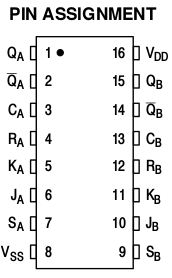
\includegraphics[scale=.4]{pin}
\caption{Zoccolatura del 14027}
\label{fig:pin}
\end{figure}

\begin{figure}[htp]
\centering
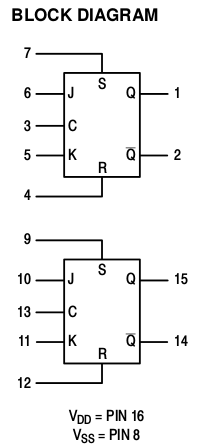
\includegraphics[scale=.4]{scheme}
\caption{Definizione dei pin}
\label{fig:defpin}
\end{figure}

In figura \ref{fig:times} sono definiti i tempi di risposta per gli ingressi J,K e il CLOCK con S e R nello stato 0, mentre in figura \ref{fig:srtimes} sono mostrati i tempi di risposta con S e R variabili.

\begin{figure}[htp]
\centering
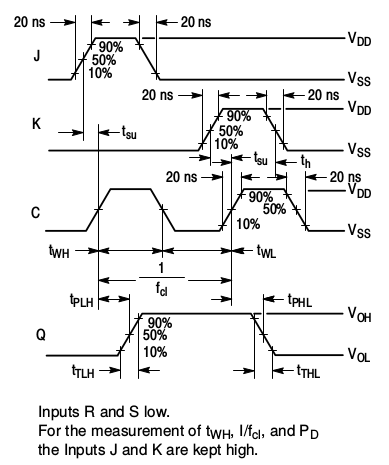
\includegraphics[scale=.4]{times}
\caption{Definizione dei tempi di risposta con S e R bassi}
\label{fig:times}
\end{figure}

\begin{figure}[htp]
\centering
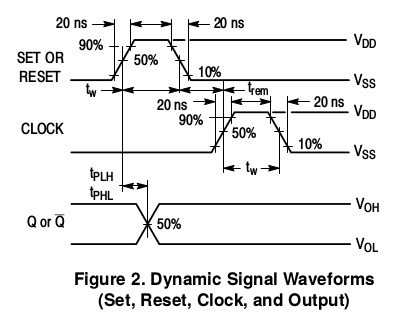
\includegraphics[scale=.4]{srtimes}
\caption{Definizione dei tempi di risposta con S e R variabili}
\label{fig:srtimes}
\end{figure}

In tabella \ref{tab:val} e \ref{tab:data} sono elencati rispettivamente i valori tipici di corrente, alimentazione e consumo e le fasce di tensione del 14027, del tutto identiche a quelle del \emph{flip-flop} D.

\begin{table}[htp]
\centering
\caption{Valori tipici del 14027.}
\label{tab:val}
\begin{tabular}{|c|c|}
\hline 
Grandezza & Valore \\ 
\hline 
Tensione di alimentazione & $V_{min} = -0.5 V$, $V_{max} = 18 V$ \\ 
\hline 
Input current & 10 mA \\ 
\hline 
Consumo massimo & 500 mW \\ 
\hline 
\end{tabular} 
\end{table}

\begin{table}[htp]
\centering
\caption{Fasce di tensione del 14027}
\label{tab:data}
\begin{tabular}{|c|c|c|}
  \hline
  Grandezza & $V_{DD}$ (V)& Valore \\
  \hline
           &  5  &  0.05 V \\ \cline{2-3}
  $V_{OL}$ & 10  &  0.05 V \\ \cline{2-3}
           & 15  &  0.05 V \\ 
  \hline 
           &  5  &  4.95 V \\ \cline{2-3}
  $V_{OH}$ & 10  &  9.95 V \\ \cline{2-3}
           & 15  & 14.95 V \\ 
  \hline \hline
           &  5  &  1.5 V \\ \cline{2-3}
  $V_{IL}$ & 10  &  3.0 V \\ \cline{2-3}
           & 15  &  4.0 V \\ 
  \hline 
           &  5  &  3.5 V \\ \cline{2-3}
  $V_{IH}$ & 10  &  7.0 V \\ \cline{2-3}
           & 15  &   11 V \\ 
  \hline
\end{tabular}
\end{table}

In figura \ref{fig:truth} è mostrata la tavola di verità del JK. Si può notare come per S e R non entrambi nulli e per segnale di clock decrescente le uscite siano identiche al \emph{flip-flop} D; invece per S=R=0 la presenza di un ingresso aggiuntivo comporta delle differene sostanziali, in particolare per la configurazione J=K=1 con clock crescente è previsto lo switch delle uscite.

\begin{figure}[htp]
\centering
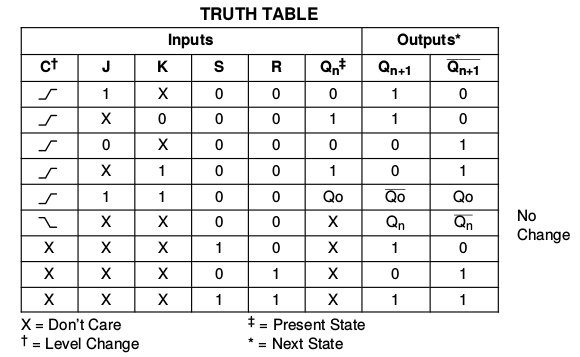
\includegraphics[scale=.4]{truthtable}
\caption{Tavola di varità del \emph{flip-flop} JK}
\label{fig:truth}
\end{figure}

In laboratorio abbiamo verificato che il 14027 impiegato riproducesse la tavola di verità di figura \ref{fig:truth} tramite tester digitale per tutte le combinazioni possibili di S, R, J e K, in particolare abbiamo verificato che per J=K=1 il \emph{flip-flop} si comportasse come un divisore per 2.

\section{Divisore per 3}

Come prima applicazione del \emph{flip-flop} JK abbiamo studiato il divisore per 3 realizzando il circuito in figura \ref{fig:div3}.

\begin{figure}[htp]
\centering
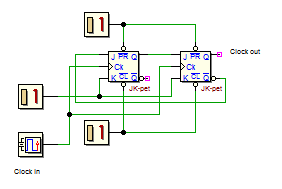
\includegraphics[scale=0.95]{es3}
\caption{Schema del divisore per 3}
\label{fig:div3}
\end{figure}

A partire dalla tavola di verità \ref{fig:truth} è possibile dedurre la sequenza degli stati del circuito, come si vede in tabella \ref{tab:div3}.

\begin{table}[htp]
\centering
\caption{Sequenza degli stati per il divisore}
\label{tab:div3}
\begin{tabular}{|c|c|c|c|}
\hline 
J1 & Q1 & Q2 & Clock \\ 
\hline 
1 & 0 & 1 & $\uparrow$ \\ 
\hline 
0 & 0 & 1 & $\downarrow$ \\ 
\hline 
0 & 0 & 0 & $\uparrow$ \\ 
\hline 
1 & 0 & 0 & $\downarrow$ \\ 
\hline 
1 & 1 & 0 & $\uparrow$ \\ 
\hline 
1 & 1 & 0 & $\downarrow$ \\ 
\hline 
1 & 0 & 1 & $\uparrow$ \\ 
\hline 
\end{tabular} 
\end{table}

Come si nota la prima e l'ultima riga coincidono, per cui si ottiene un ciclo. Il periodo è tre volte quello di clock, per cui a livello di tavola di verità il circuito si comporta come un divisore per 3 e ci si aspetta un duty cycle di $1/3$. Sempre dalla tabella \ref{tab:div3} si vede come lo  stato in cui Q1 = Q2 = 1 non si realizza mai, per cui esso rappresenta uno stato non utilizzato. Inoltre è evidente che non esistono stati non raggiungibili, infatti il circuito possiede due gradi di libertà iniziali, ovvero due ingressi che possono essere settati liberamente, e che possono essere rappresentati da J1 e Q1. Pertanto esistono 4 stati iniziali corrispondenti alle coppie (1,1), (0,0), (1,0), (0,1), di cui i primi 3 effettivamente si riscontrano, mentre l'ultimo sparisce quando il clock si trova nello ''stato'' up, in quanto Q1 assume valore 0 facendo entrare lo stato del circuito dentro il ciclo. L'evoluzione del circuito si può rappresentare graficamente come in figura \ref{fig:graph}, in cui si vede come lo stato (1,1) non compare all'interno del ciclo, rimnendo quindi non utilizzato.\\

\begin{figure}[htp]
\centering
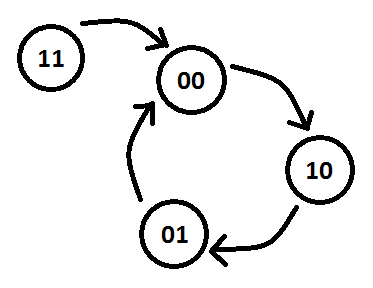
\includegraphics[scale=.5]{Immagine}
\caption{Stati in uscita dal divisore per 3}
\label{fig:graph}
\end{figure}

Abbiamo realizzato effettivamente il circuito collegando l'ingresso del clock al \emph{digital output} 47 e impiegando il VI \texttt{Digital$\_$out4} per generare il segnale, abbiamo collegato le uscite Q1 e Q2 al tester digitale a abbiamo verificato che effettivamente il circuito riproducesse la sequenza di stati previsti.\\
Abbiamo studiato la risposta del circuito collegandolo al generatore di funioni ATTEN, impostando come frequenza di clock 3 kHz. Abbiamo impiegato il fedele VI \texttt{ACQUIS$\_$BASE$\_$2015} e in figura \ref{fig:vi} si può vedere l'esito della misura. Come si può notare il circuito si comporta ancora come divisore per 3 e anche il valore del duty cycle è quello ottenuto precedentemente.

\begin{figure}[htp]
\centering
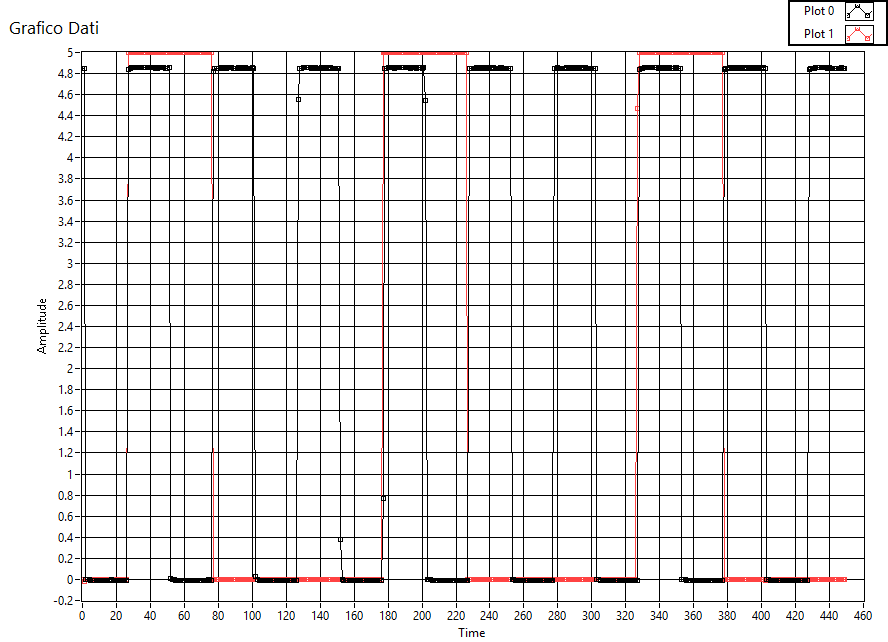
\includegraphics[scale=.25]{es7_sym}
\caption{Confronto fra il segnale di clock (nero) e l'uscita del divisore (rosso)}
\label{fig:vi}
\end{figure}

Per verificare quantitativamente le precedenti affermazioni abbiamo impiegato i VI \texttt{Contatore$\_$freq} e \texttt{Contatore$\_$pulsew}. Tramite il primo VI abbiamo effettuato le misure dei periodi/frequenze dei segnali in ingresso e in uscita, mentre con il secondo VI abbiamo misurato il duty cycle del segnale in uscita al divisore, in entrambi i casi considerando una popolazione statistica di 100 campioni. In tabella \ref{tab:es6-1} e \ref{tab:es6-2} sono mostrati i risultati relativi alle misure di frequenza in ingresso e in uscita, rispettivamente compatibili con i valori impostati e attesi di 3 kHz e 1 kHz. In tabella \ref{tab:es6-3} è mostrata la durata dello stato 1 sul segnale in uscita che è compatibile con $1/3$ del periodo misurato in tabella \ref{tab:es6-2}, per cui il duty cycle del segnale in uscita dal nostro divisore è quello previsto.

\begin{table}[htp]
\centering
\caption{Frequenze e periodi dei segnali in ingresso}
\label{tab:es6-1}
\begin{tabular}{|c|c|c|}
\hline
Grandezza & Valore & Campioni\\
\hline 
Frequenza & 2999.86 Hz & 72 \\ \cline{2-3}
          & 3000.29 Hz & 28 \\ 
\hline 
Periodo & 0.333301 ms & 27 \\ \cline{2-3}
        & 0.333349 ms & 73 \\ 
\hline 
\end{tabular} 
\end{table}

\begin{table}[htp]
\centering
\caption{Frequenze e periodi dei segnali in uscita}
\label{tab:es6-2}
\begin{tabular}{|c|c|c|}
\hline
Grandezza & Valore & Campioni\\
\hline 
Frequenza & 999.951 Hz & 23 \\ \cline{2-3}
          & 999.999 Hz & 77 \\ 
\hline 
Periodo & 1 ms & 80       \\ \cline{2-3}
        & 1.00005 ms & 20 \\ 
\hline 
\end{tabular} 
\end{table}

\begin{table}[htp]
\centering
\caption{Misura duty cycle}
\label{tab:es6-3}
\begin{tabular}{|c|c|c|}
\hline
Tempo  & 0.333351 ms & 64 \\ \cline{2-3}
       & 0.333399 ms & 36 \\ 
\hline 
\end{tabular} 
\end{table}

Ovviamente non è possibile variare il segnale di clock per ottenere un segnale in uscita dal divisore con duty $1/2$ dal momento che ciò che determina la variazione dello stato del circuito è il cambiamento dello stato del clock e non la sua permanenza in uno stato 0 o 1.

\section{Simmetrizzatore}
Avendo ottenuto facilmente un divisore per tre con due integrati \textsc{jk}, possiamo ora provare, come nella precedente esperienza, a \textit{simmetrizzare} il segnale di uscita \textsc{qb} montando un circuito simmetrizzatore composto da un flip-flop D-type e un integrato \textbf{NOR}, \textsc{hc02}, come mostrato in Figura (\ref{fig:es15_simmet}).\\
Contrariamente alla volta precedente, però, bisogna fare attenzione al fatto che il segnale in uscita \textsc{qb} da simmetrizzare ha duty cycle $\eta = 1/3$, e \underline{non} più $\eta = 2/3$ (in altre parole la sequenza è 001001 invece che 110110): come conseguenza di questo fatto, per ottenere in uscita un $\eta = 1/2$ bisogna connettere \textsc{qb} (porta 15) con l'ingresso del \textbf{NOR} e \textsc{$\neg$qb} (porta 14) con la porta 5 (ingresso D) del flip-flop. In caso contrario ci saremmo aspettati ragionevolmente un duty di 1/6. In effetti questi sono proprio i risultati che otteniamo analizzando in primo luogo con il \textit{VI} \textsc{acquis\_base2} il segnale \textsc{qb} e l'uscita del \textbf{NOR}, rispettivamente collegati alla \textsc{cb68} e alla \textsc{cb33}, e infine con il \textit{VI} \textsc{pulse\_w} collegando la \textsc{cb3} separatamente ai due segnali.\\
Il generatore di funzioni è stato impostato ad una frequenza di 3kHz, con una tensione picco-picco $V_{pp} = 5V$ e un offset $V_{off} = +2.5V$. Le porte e i collegamenti dei circuiti sono riportati in Figura (\ref{fig:simm_div_3}) per il caso 15->D, invece i valori ottenuti dei \textit{duty-cycle} sono i seguenti:\\

\begin{table}[h]
\centering
\begin{tabular}{c|c|c}
\hline  & rising-time (ms) & duty-cycle $\eta$\\ 
\hline 15 $\rightarrow$ NOR, 14$\rightarrow$ D & 0.49999(5) & 0.5000(1) \\ 
\hline 15 $\rightarrow$ D, 14 $\rightarrow$ NOR & 0.16670(5) & 0.16670(7) \\ 
\hline
\end{tabular} 
\end{table}
~\\

\begin{figure}
\centering
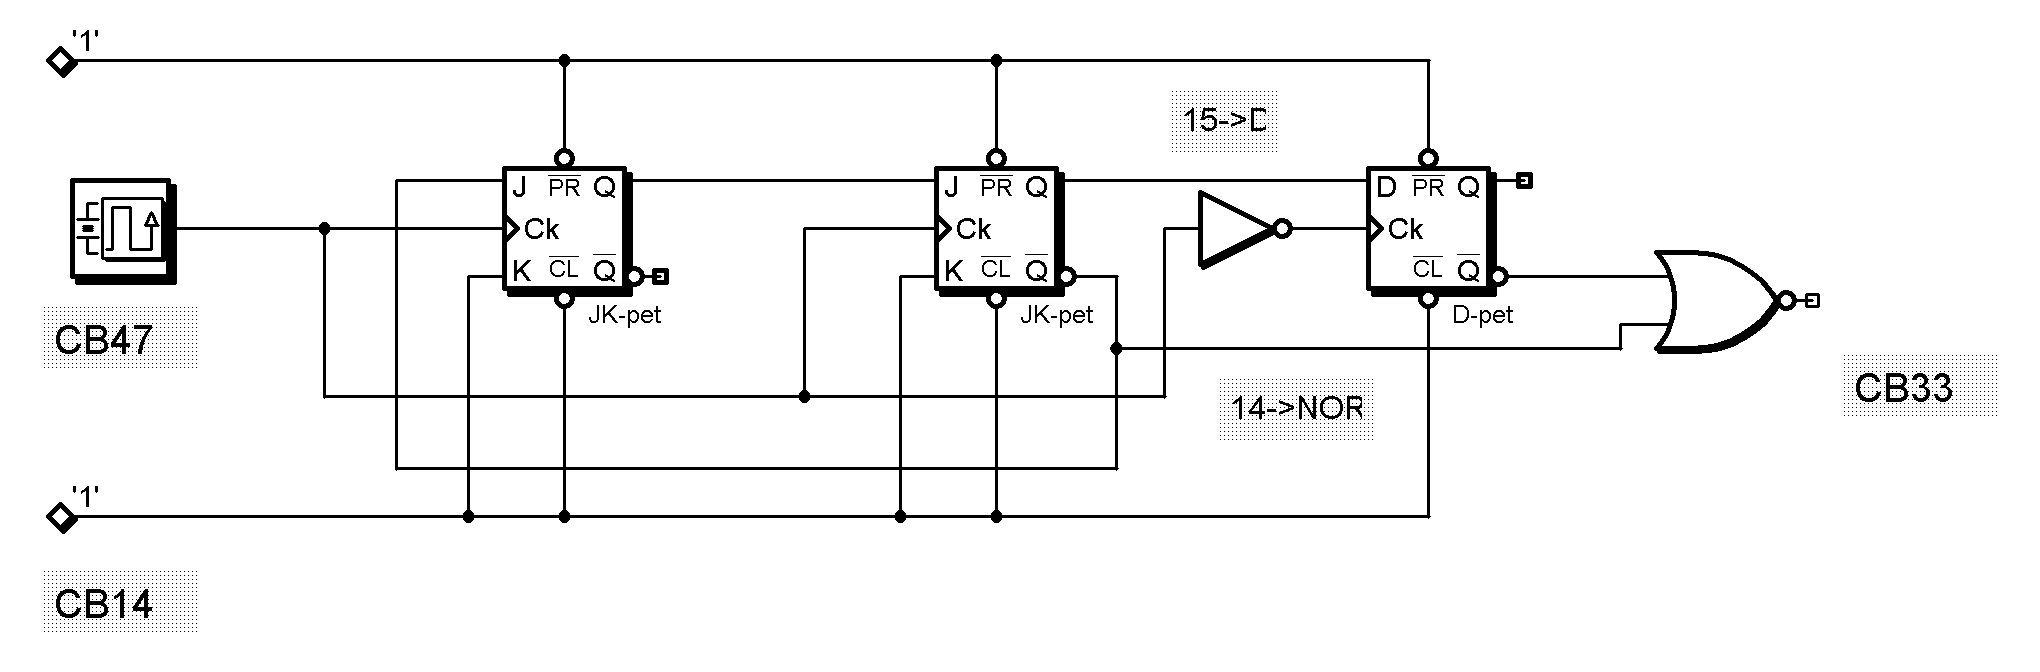
\includegraphics[width=0.8\linewidth]{./simm_div_3}
\caption{Schema circuitale del divisore per tre + simmetrizzatore (parte a dx della figura). Questa configurazione produce un $\eta = 1/6$.}
\label{fig:simm_div_3}
\end{figure}


\begin{figure}
\centering
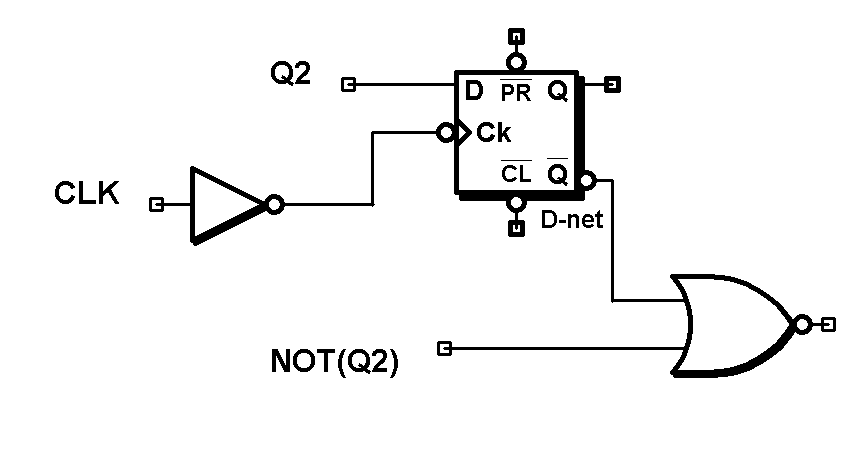
\includegraphics[width=0.8\linewidth]{./es15_simmet}
\caption{Circuito simmetrizzatore}
\label{fig:es15_simmet}
\end{figure}

Nei grafici in Figura (\ref{fig:es9_simmetrizzatore_15nor_14d}, \ref{fig:es9_simmetrizzatore_14nor_15d}) sono riportate le acquisizioni di \textsc{acquis\_base2}.

\begin{figure}
\centering
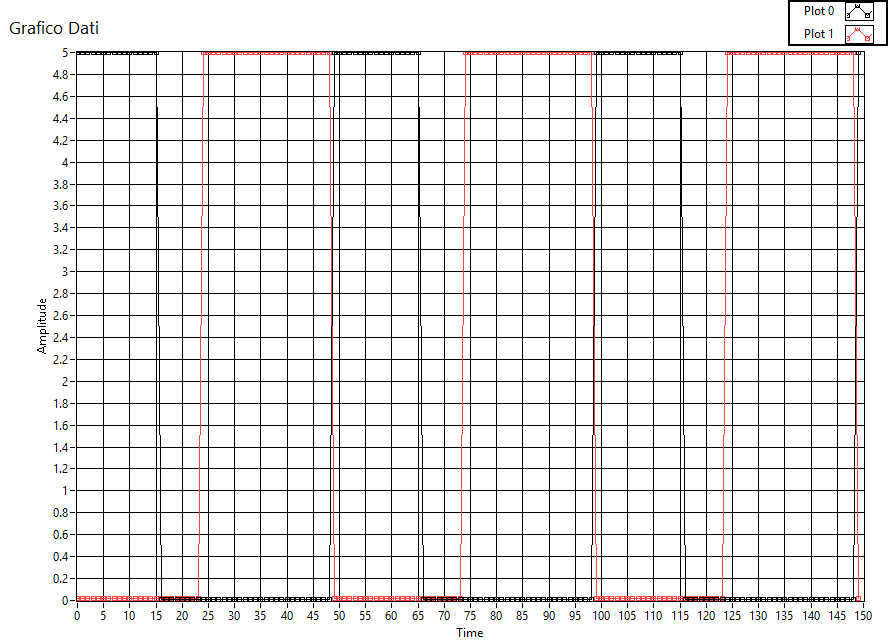
\includegraphics[width=0.8\linewidth]{./es9_simmetrizzatore_15nor_14d.png}
\caption{Segnale simmetrizzato (15- $\rightarrow$ NOR, 14- $\rightarrow$D)}
\label{fig:es9_simmetrizzatore_15nor_14d}
\end{figure}

\begin{figure}
\centering
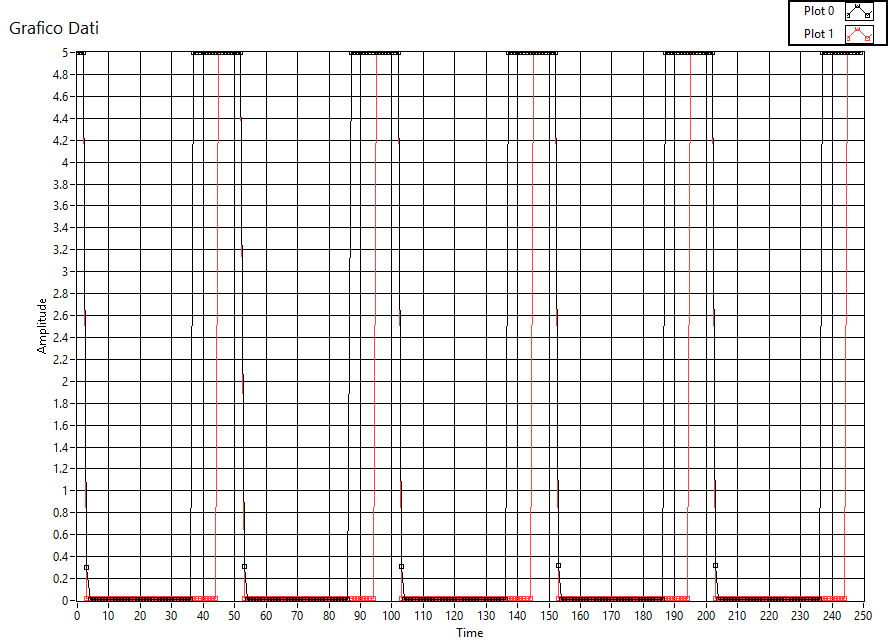
\includegraphics[width=0.8\linewidth]{./es9_simmetrizzatore_14nor_15d}
\caption{Segnale non simmetrizzato (14- $\rightarrow$ NOR, 15- $\rightarrow$D), duty-cycle = 1/6}
\label{fig:es9_simmetrizzatore_14nor_15d}
\end{figure}

\subsection{Hw.2}
Ci chiediamo ora che tipo di segnale otterremmo se al posto del circuito \textbf{NOR} usassimo un \textbf{NAND}. Per le stesse ragioni di "\textit{simmetria}" presentate nel logbook della scorsa esperienza, che discendono dal confronto della tavola di verità fra il \textbf{NOR} e il \textbf{NAND} riportata di seguito, ci aspettiamo che si invertano i segnali di uscita con duty di 1/2 e 1/6 in base a dove va la porta 15 \textsc{qb} nel circuito simmetrizzatore. Per essere più chiari: questa volta 15 $\rightarrow$D e 14 $\rightarrow$NOR avrà in uscita il segnale simmetrico con duty-cycle 1/2 e non più quello con $\eta = 1/6$.\\


\begin{table}[h]
\centering
\begin{tabular}{c|c||c|c}
\hline \textbf{A} & \textbf{B} & \textbf{NAND(A,B)} & \textbf{NOR(A,B)} \\ 
\hline 1 & 1 & 0 & 0 \\ 
 1 & 0 & 1 & 0 \\ 
 0 & 1 & 1 & 0 \\ 
 0 & 0 & 1 & 1 \\ 
\hline
\end{tabular} 
\end{table}
~\\

Per verificarlo scriviamo la tavola di verità nel caso in cui 15- $\rightarrow$D:

\begin{table}[h] %15- $\rightarrow$D
\centering
\begin{tabular}{c|c|c|c|c|cl}
\hline \textbf{CLK} & \textbf{QB=D} & \textbf{Q} & \textbf{$\lnot Q$} & \textbf{$\lnot QB$} & \textbf{NOR($\lnot QB, \lnot Q1)$} & \textbf{NAND($\lnot QB, \lnot Q1)$}\\ 
\hline
 1 & 1 &   -&  -& 0 & -& \\ 
 0 & 1 &   1&  0& 0 & 1& 1\\
 1 & 0 &   1&  0& 1 & 0& 1\\ 
 0 & 0 &   0&  1& 1 & 0& 0\\ 
 1 & 0 &   0&  1& 1 & 0& 0\\
 0 & 0 &   1&  0& 1 & 0& 1\\
 1 & 1 &   1&  0& 0 & 1& 1\\
\end{tabular} 
\end{table}
~\\

I risultati soddisfano le nostre aspettative sia nel caso 15 $\rightarrow$D ($\eta = 1/2$) che in quello (non riportato) 14 $\rightarrow$D ($\eta = 1/6$).

\section{Contatore decimale}
Combinando opportunamente quattro \textit{flip-flop} \textsc{jk} con dei circuiti \textbf{AND}, è possibile realizzare un contatore decimale a codifica binaria. Lo schema del circuito (già semplificato) è riportato in Figura (\ref{fig:dec_counter}).\\

\begin{figure}
\centering
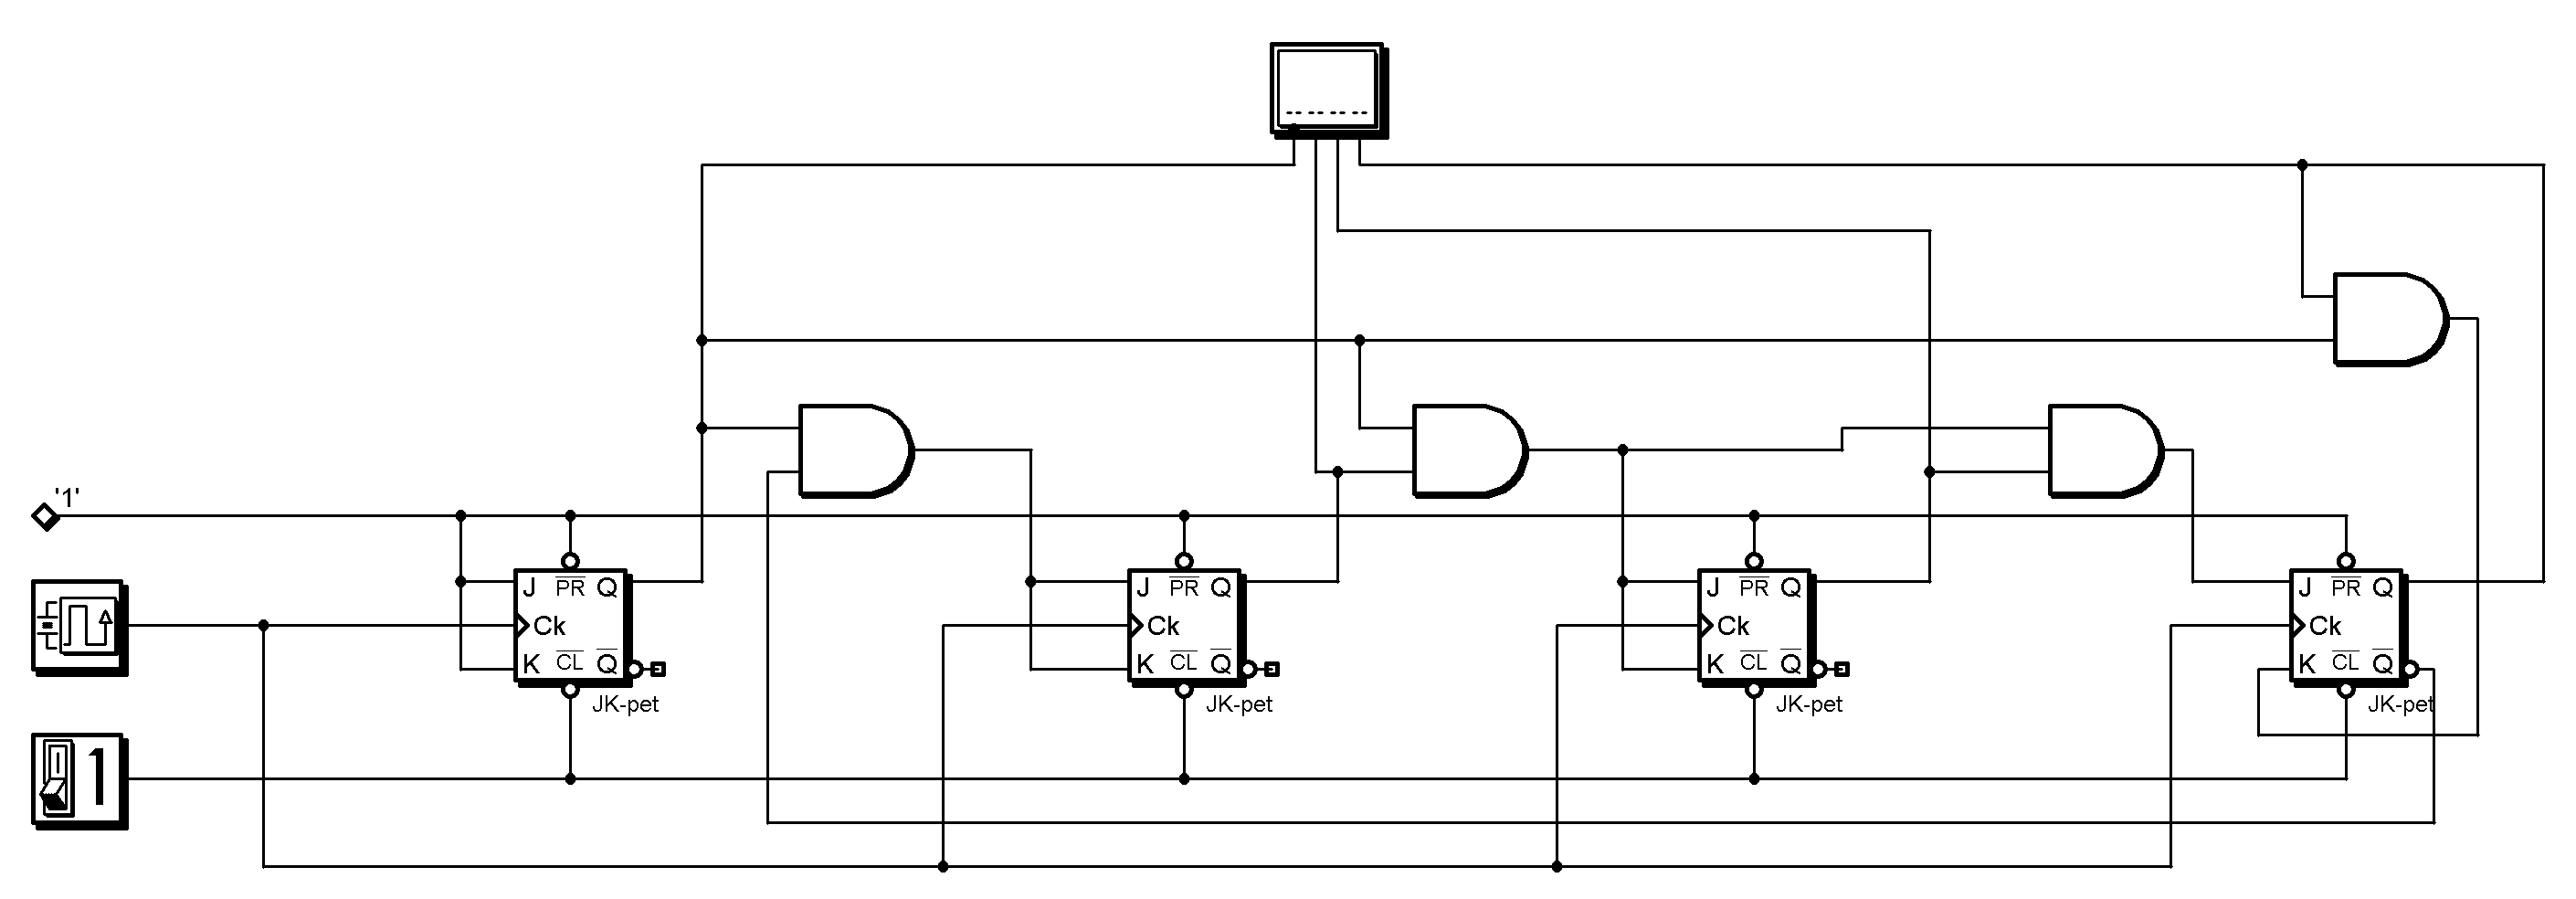
\includegraphics[width=0.9\linewidth]{./dec_counter}
\caption{Schema del contatore decimale binario}
\label{fig:dec_counter}
\end{figure}


%La sequenza di stati di tale circuito per ogni fronte di risalita del clock può essere riassunta nella seguente tabella, definendo con i pedici A,B,C,D le porte rispettivamente del primo, del secondo, del terzo e del quarto integrato \textsc{jk}:
%
%\begin{tabular}{|c|c|c|c|c|c|c|c|c|c|c|c|}
%\hline $J_A$ & $K_A$ & $Q_A$ & $J_B$ & $K_B$ & $Q_B$ & $J_C$ & $K_C$ & $Q_C$ & $J_D$ & $K_D$ & $Q_D$ \\ 
%\hline 1 & 1 & 1 & 1 & 1 & 0 & 0 & 0 & 0 & 0 & 0 & 0 \\ 
%\hline 1 & 1 & 0 & 0 & 0 & 1 & 0 & 0 & 0 & 0 & 0 & 0 \\ 
%\hline 1 & 1 & 1 & 1 & 1 & 1 & 1 & 1 & 0 & 0 & 0 & 0 \\ 
%\hline 1 & 1 & 0 & 0 & 0 & 0 & 0 & 0 & 1 & 0 & 0 & 0 \\ 
%\hline 1 & 1 & 1 & 1 & 1 & 0 & 0 & 0 & 1 & 0 & 0 & 0 \\ 
%\hline 1 & 1 & 0 & 0 & 0 & 1 & 0 & 0 & 1 & 0 & 0 & 0 \\ 
%\hline 1 & 1 & 1 & 1 & 1 & 1 & 1 & 1 & 1 & 1 & 0 & 0 \\ 
%\hline 1 & 1 & 0 & 0 & 0 & 0 & 0 & 0 & 0 & 0 & 0 & 1 \\ 
%\hline 1 & 1 & 1 & 0 & 0 & 0 & 0 & 0 & 0 & 0 & 1 & 1 \\ 
%\hline 
%\end{tabular} 


Concretamente, il circuito pone alcune sfide nella realizzazione dovute al numero di circuiti da impiegare e al fatte che a nostra disposizoone ci sono degli integrati \textbf{NAND} e non \textbf{AND}, motivo per cui bisognerà corocircuitare ogni volta due ingressi in più e gestire altri cavetti di cui non se ne sentiva la mancanza. Per montare con meno problemi possibile il contatore decimale, è stato impiegato uno schema realizzativo come quello in Figura (\ref{fig:circuito_counter_up}). Organizzati in questo modo, il circuito ha funzionato al primo colpo!\\

Concentriamoci ora sulla sequenza degli stati del sistema, andando ad osservare le quadruplette (Q4,Q3,Q2,Q1) per ricercare gli stati irrangiungibili e/o inutilizzati.

\begin{table}[h]
\centering
\begin{tabular}{l|l|l|l}
\textbf{q4} &\textbf{ q3} & \textbf{q2} & \textbf{q1} \\
\hline
0 & 0 & 0 & 0 \\

0 & 0 & 0 & 1 \\

0 & 0 & 1 & 0 \\

0 & 0 & 1 & 1 \\

0 & 1 & 0 & 0 \\

0 & 1 & 0 & 1 \\

0 & 1 & 1 & 0 \\

0 & 1 & 1 & 1 \\

1 & 0 & 0 & 0 \\

1 & 0 & 0 & 1 \\

0 & 0 & 0 & 0 \\
\hline
\end{tabular}
\end{table}
~\\

Questa è dunque la sequenza periodica degli stati (Q4,Q3,Q2,Q1), ponendo come condizione iniziale i valori (0,0,0,0). Si tratta, ovviamente, di solo 10 dei 16 stati ottenibili complessivamente. E' allo stesso tempo evidente che questi stati mancanti non vengono mai raggiunti una volta entrati nel ciclo principale (0,0,0,0) $\rightarrow$(1,0,0,1), per cui, se vengono effettivamente raggiunti almeno una volta, ciò avverrà prima di inserirsi nella sequenza principale, e dipenderà dalle condizioni iniziali.\\

\textsc{avvertenza}: per analizzare in dettaglio il comportamento di questo e della gran parte degli altri circuiti presentati nel logbook, con tutti gli stati raggiungibili, inutilizzabili (ecc...), abbiamo proceduto a simulare l'integrato \textsc{jk} in Python, definendo una funzione apposita \textsc{jk(jk(clk, j0, k0, q0))} come riportata di seguito:

def jk(clk, j0, k0, q0):\\
    if (clk == 1):\\
        if (j0 != k0):\\
            return [j0, k0, j0] \\
        elif ((j0== 0) \& (k0 == 0)):\\
            return [j0, k0, q0]\\
        else:\\
            return [j0, k0, (q0+1)%2] #q0 negato\\
    else:\\
        return [j0, k0, q0]\\

Un circuito come il contatore decimale è stato ottenuto collegando in sequenza più \textsc{jk}, ciascuno con le variabili in ingresso definite correttamente.\\

Con questi mezzi, andiamo ad osservare ora cosa succede provando ad imporre come condizioni iniziali (Q4,Q3,Q2,Q1) alcuni stati non raggiunti dal ciclo principale.\\

\begin{table}[h]
\centering
\begin{tabular}{l|l|l|l}
\textbf{q4} &\textbf{ q3} & \textbf{q2} & \textbf{q1} \\
\hline
1 & 1 & 1 & 0 \\

1 & 1 & 1 & 1 \\

0 & 0 & 1 & 0 \\

0 & 0 & 1 & 1 \\

0 & 1 & 0 & 0 \\

0 & 1 & 0 & 1 \\

0 & 1 & 1 & 0 \\

0 & 1 & 1 & 1 \\

1 & 0 & 0 & 0 \\

1 & 0 & 0 & 1 \\

0 & 0 & 0 & 0 \\
\hline
\end{tabular}
\end{table}
~\\

\begin{table}[h]
\centering
\begin{tabular}{l|l|l|l}
\textbf{q4} & \textbf{q3} & \textbf{q2} & \textbf{q1} \\
\hline
1 & 1 & 0 & 0 \\

1 & 1 & 0 & 1 \\

0 & 1 & 0 & 0 \\

0 & 1 & 0 & 1 \\

0 & 1 & 1 & 0 \\

0 & 1 & 1 & 1 \\

1 & 0 & 0 & 0 \\

1 & 0 & 0 & 1 \\

0 & 0 & 0 & 0 \\
\hline
\end{tabular}
\end{table}
~\\
\begin{table}[h]
\centering
\begin{tabular}{l|l|l|l}
\textbf{q4} & \textbf{q3} & \textbf{q2} & \textbf{q1} \\
\hline
1 & 0 & 1 & 0 \\

1 & 0 & 1 & 1 \\

0 & 1 & 1 & 0 \\

0 & 1 & 1 & 1 \\

1 & 0 & 0 & 0 \\

1 & 0 & 0 & 1 \\

0 & 0 & 0 & 0 \\
\hline
\end{tabular}
\end{table}
~\\
 
Il risultato è chiaramente visualizzabile nel grafico di Figura (\ref{fig:dec_count_graph}).


\begin{figure*}
\centering
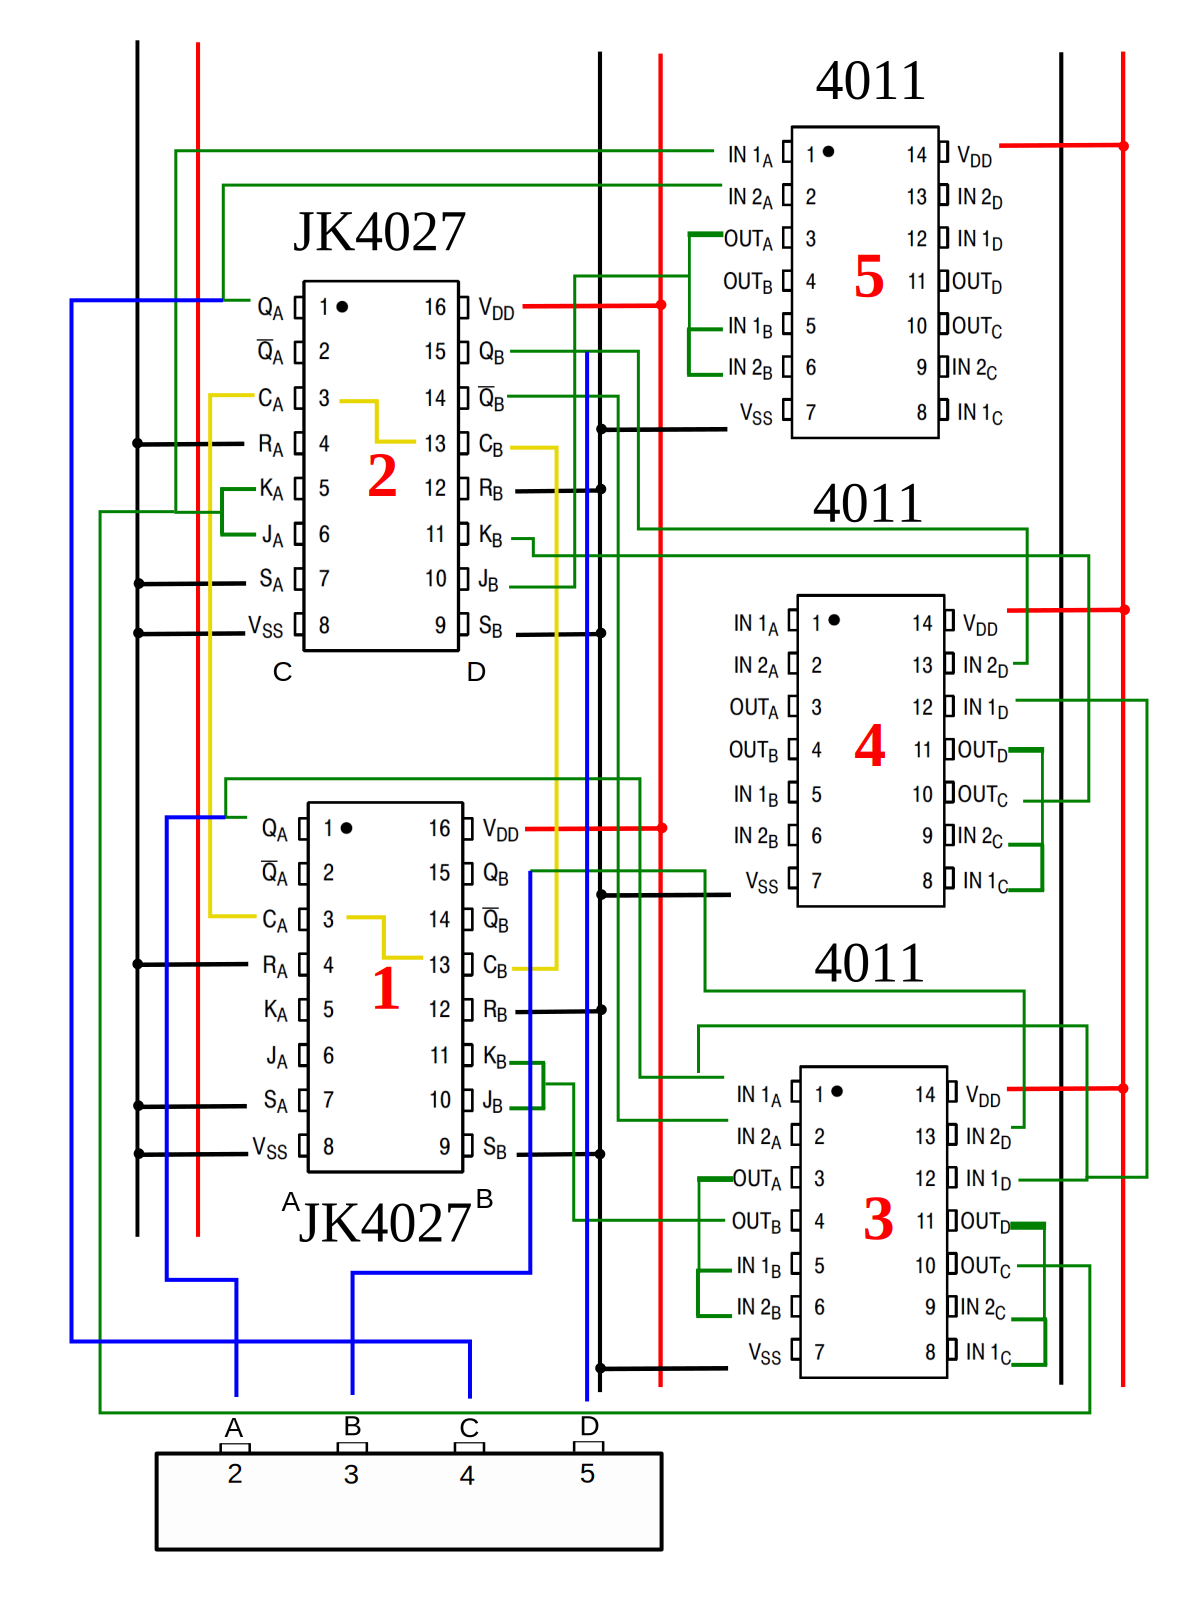
\includegraphics[width=0.8\linewidth]{./circuito_counter_up}
\caption{Schema realizzativo del contatore decimale. In giallo le linee di frequenza clock, in rosso le alimentazioni, in nero le terre, in blu le connessioni con il tester digitale e infine in verde le connessioni fra jk e NAND.}
\label{fig:circuito_counter_up}
\end{figure*}


\begin{figure}
\centering
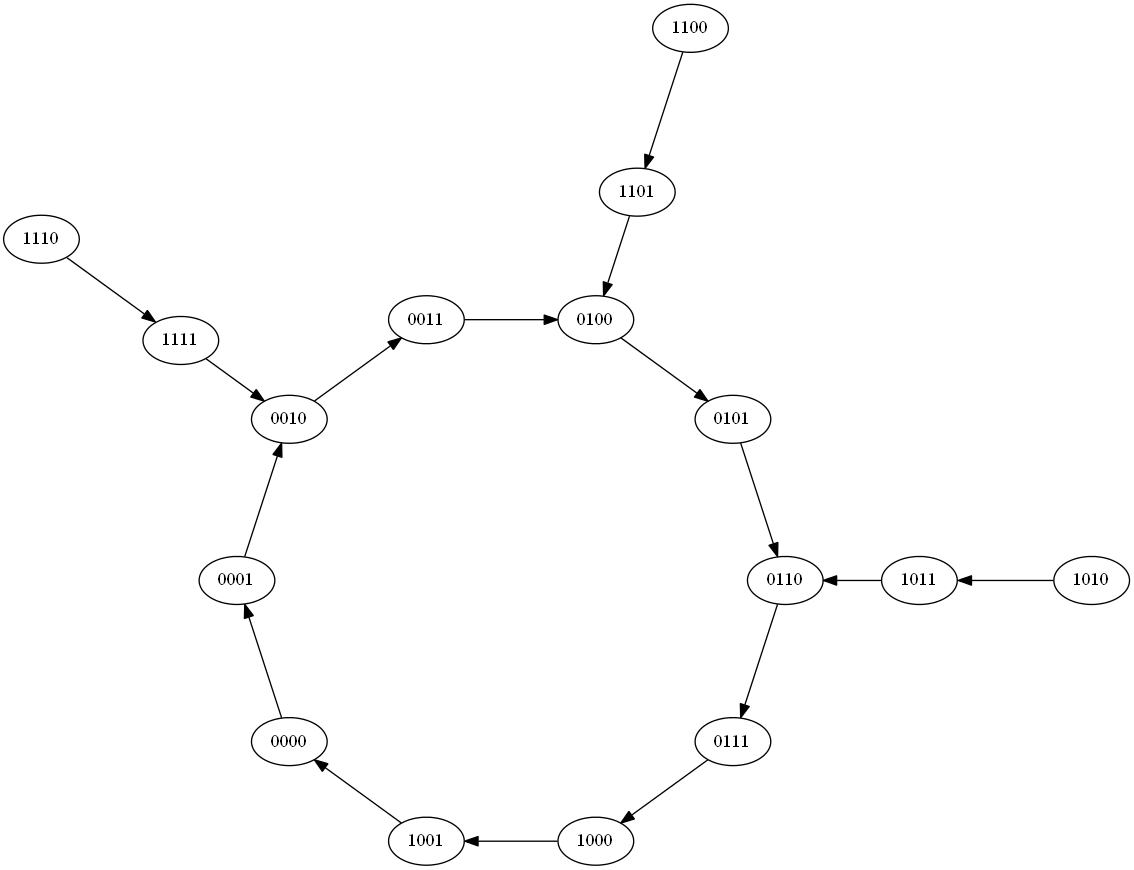
\includegraphics[width=0.9\linewidth]{./dec_count_graph}
\caption{Grafico degli stati per il contatore decimale binario}
\label{fig:dec_count_graph}
\end{figure}

\subsection{Hw. 3 - Divisore per 6}
\subsubsection{Divisori asincroni}
I circuiti analizzati fino ad ora (e quelli che analizzeremo in seguito) possono sempre essere collegati a cascata l'uno dopo l'altro. Ad esempio è possibile ottenere un divisore per sei collegando un divisore per tre in cascata ad uno per due (o viceversa), come mostrato in Figura (\ref{fig:Fig_div_6}), vale a dire collegando l'uscita a frequenza dimezzata come clock del circuito div3.\\ 
Ci aspettiamo che il duty-cycle sia $\eta = 1/3$, dato che il div2 è ovviamente simmetrico.\\


\begin{figure}
\centering
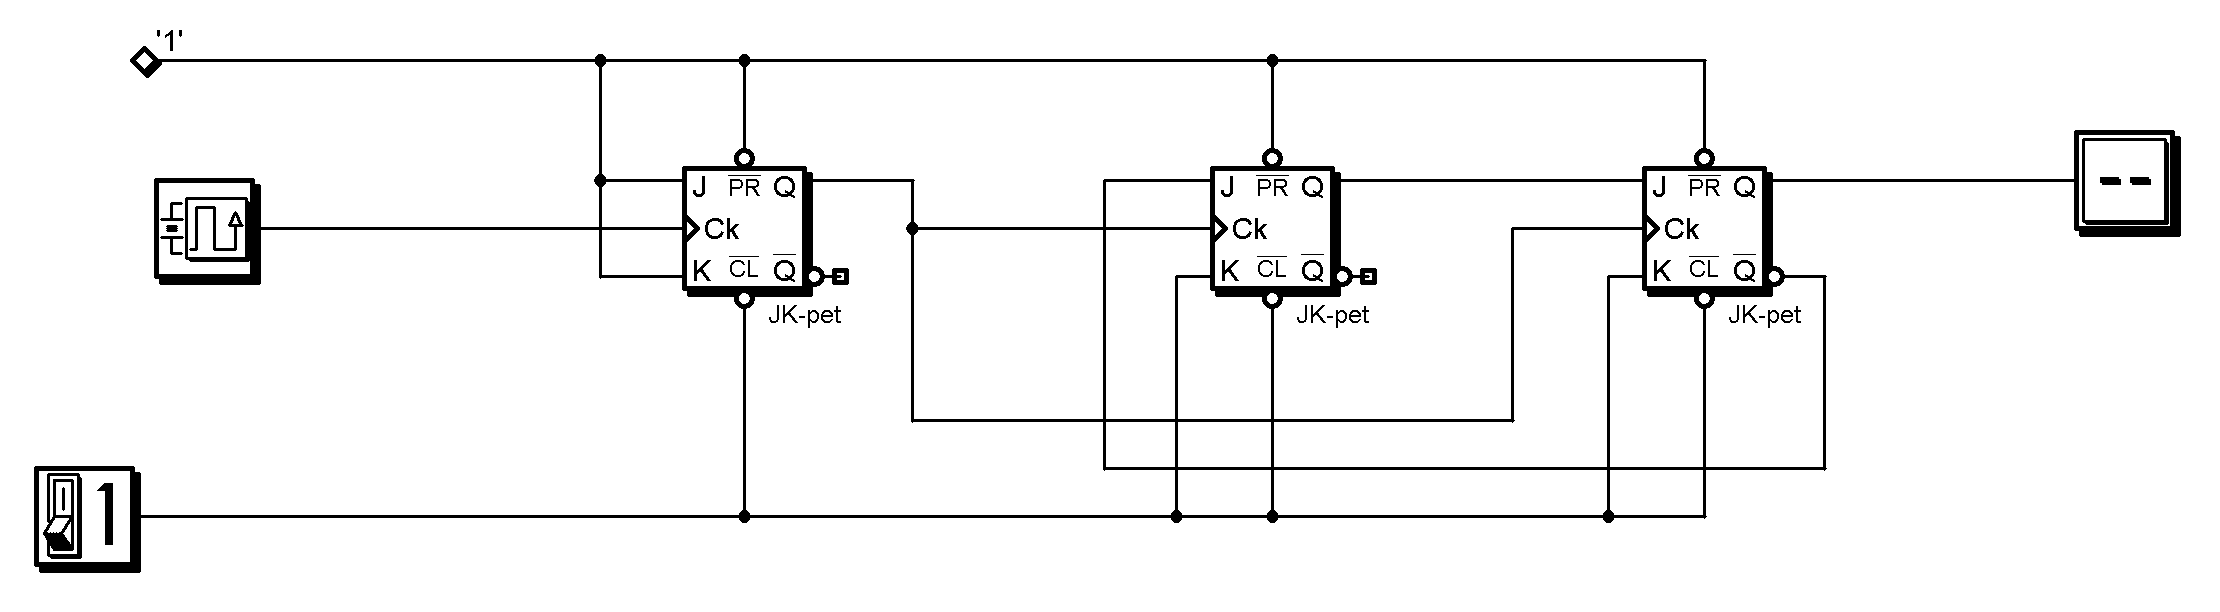
\includegraphics[width=0.8\linewidth]{./Fig_div_6}
\caption{Divisore per sei ottenuto collegando un divisore per tre in cascata ad uno per due.}
\label{fig:Fig_div_6}
\end{figure}


Alternativamente, è possibile collegare il divisore per due in cascata a quello per tre: la differenza principale che ci aspettiamo riguarda il duty-cycle, questa volta di 1/2 (Figura (\ref{fig:Fig_div_6_reverse})). In Figura (\ref{fig:div_sei_comparative_picture}) è riportata un'immagine comparativa degli stati dei divisori asincroni "ideali".\\


\begin{figure}
\centering
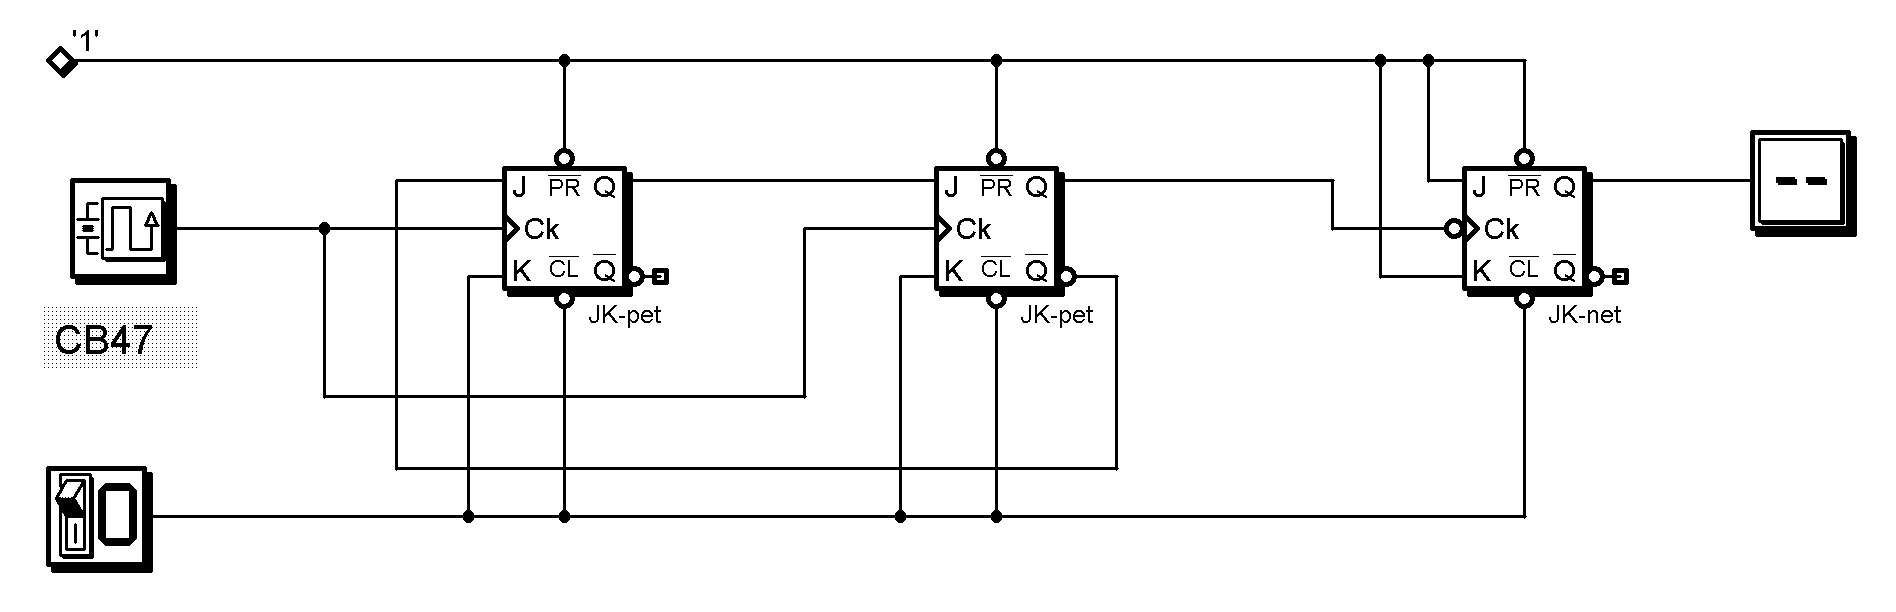
\includegraphics[width=0.8\linewidth]{./Fig_div_6_reverse}
\caption{Divisore per sei: divisore per due in cascata ad uno per tre}
\label{fig:Fig_div_6_reverse}
\end{figure}

\begin{figure}
\centering
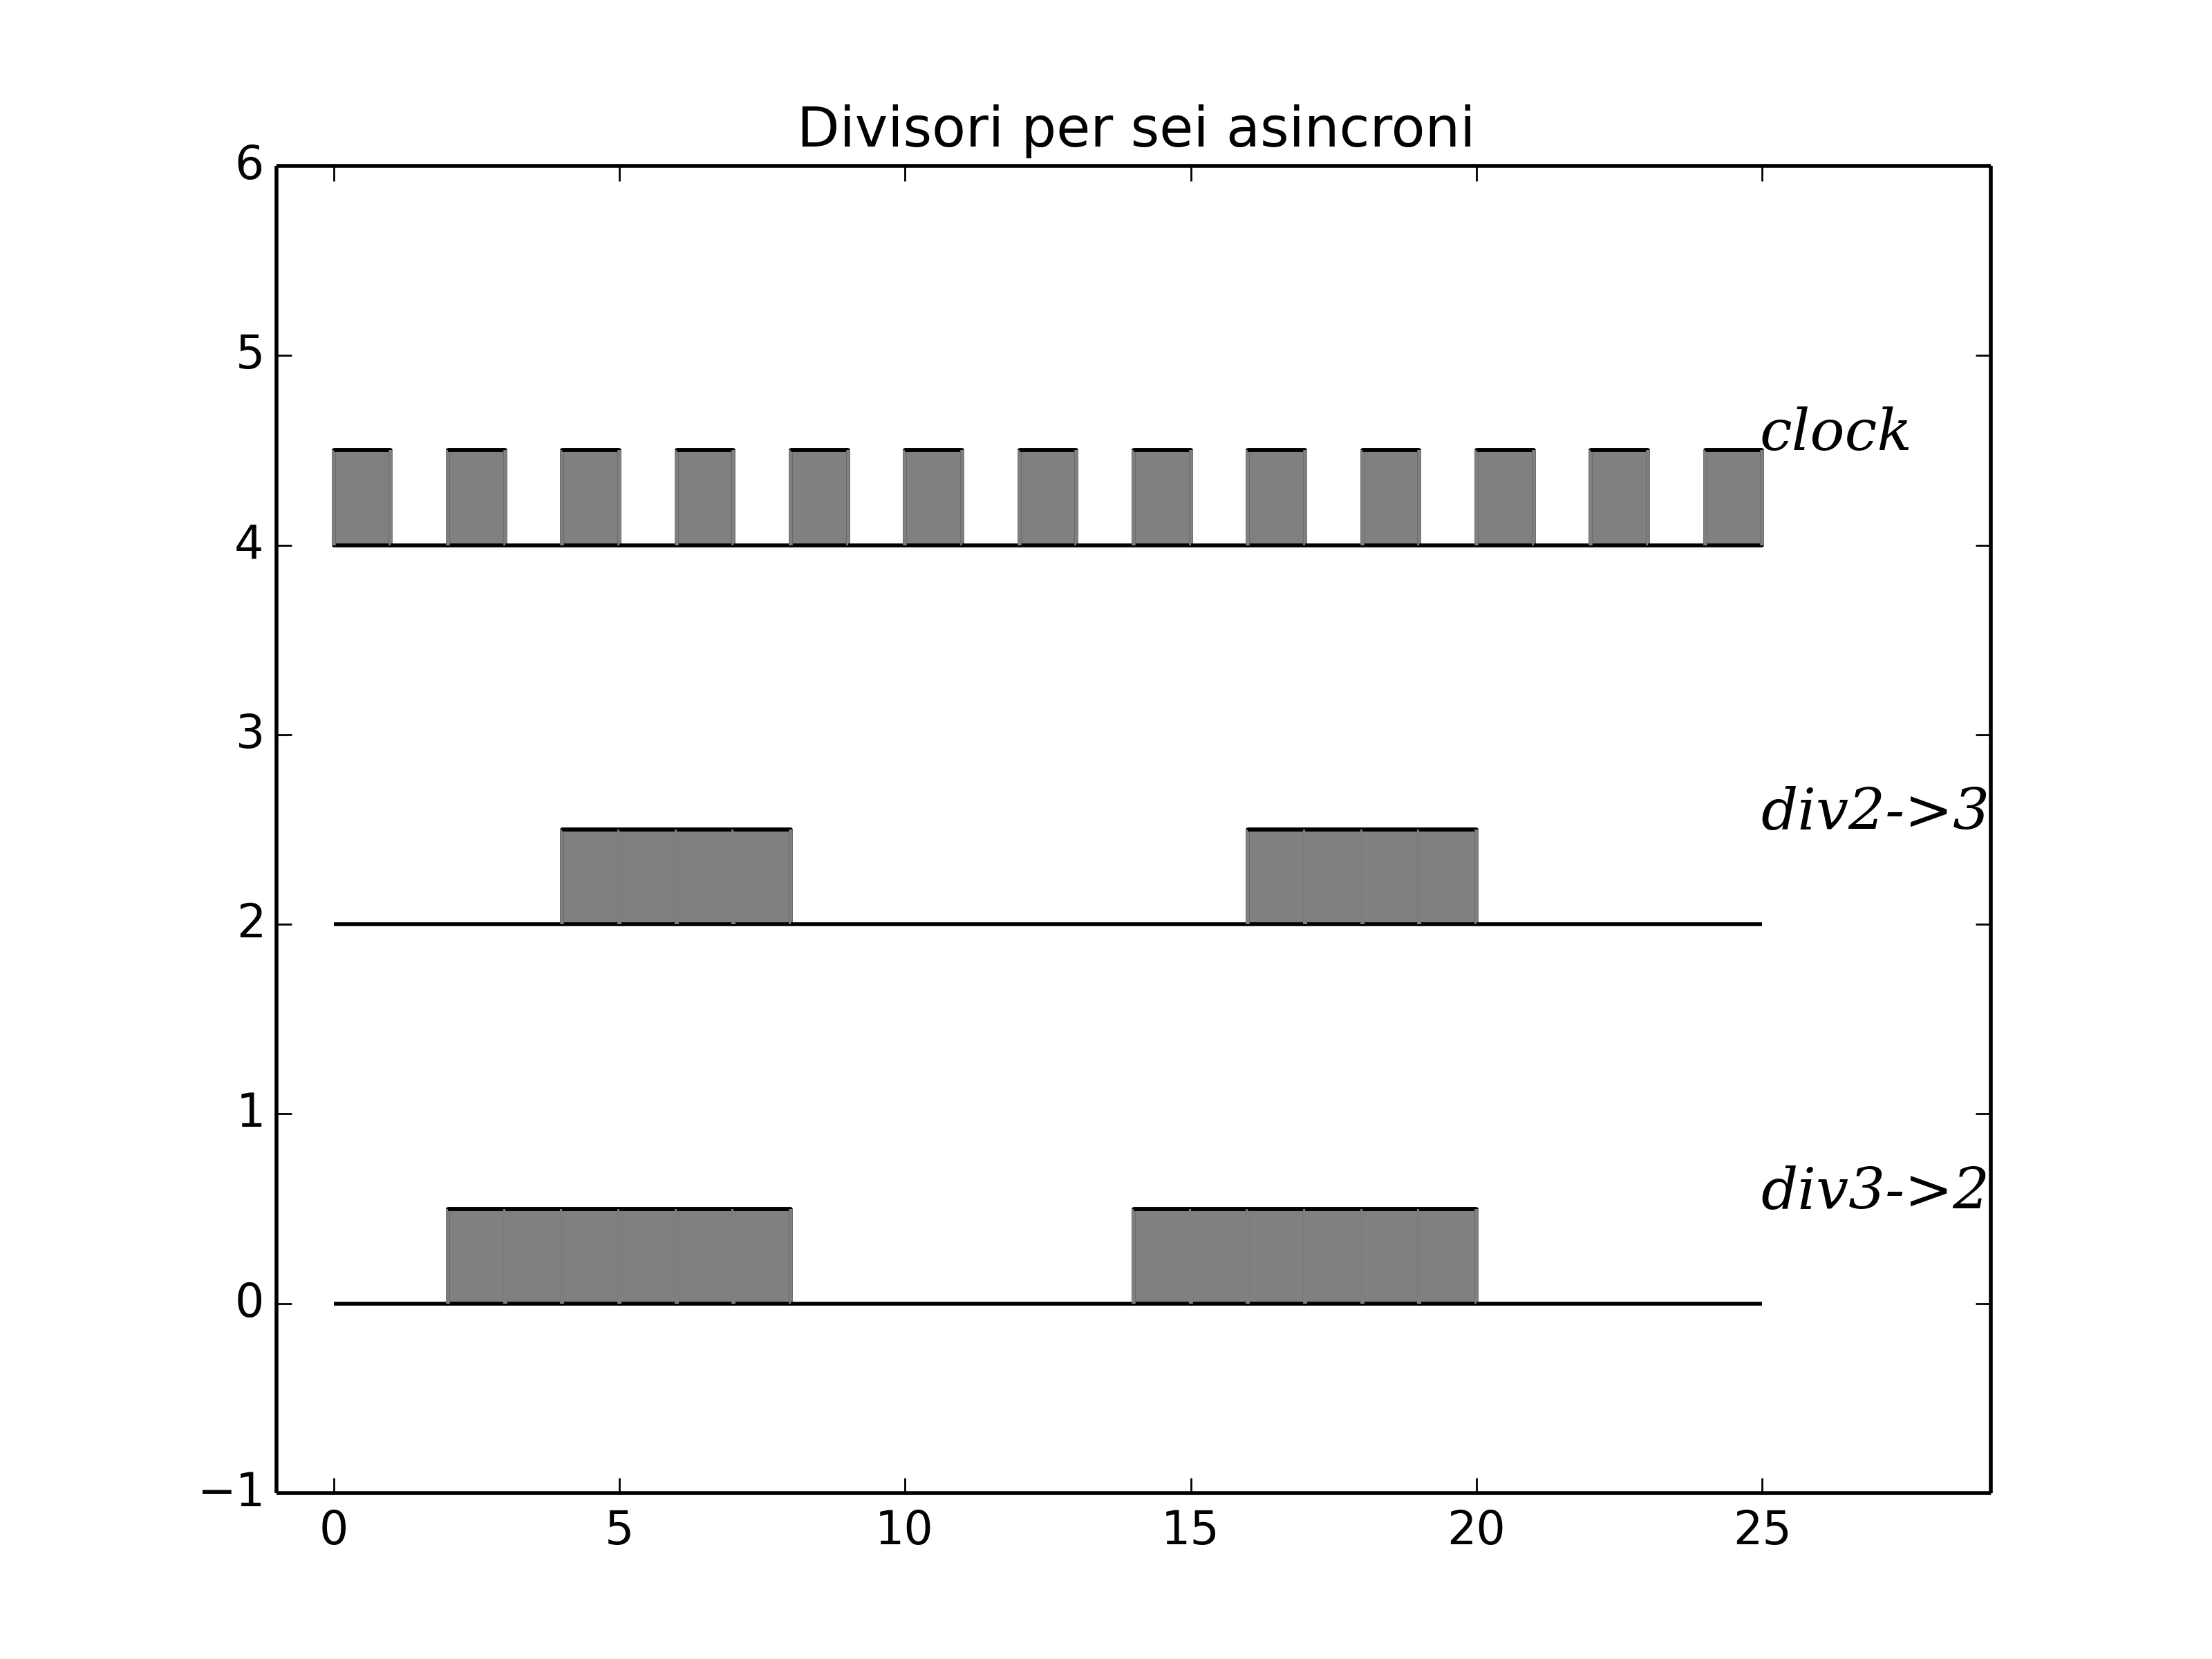
\includegraphics[width=0.9\linewidth]{./div_sei_comparative_picture}
\caption{Divisori per sei asincroni. In ordine dall'alto in basso: segnale di clock, div3 in cascata a div2, viceversa.}
\label{fig:div_sei_comparative_picture}
\end{figure}


\subsubsection{Divisore sincrono}
Lo svantaggio principale dell'utilizzo di contatori asincroni sta nel ritardo nella propagazione del segnale che dall'ingresso del clock aggiorna l'output di un integrato e che deve fare da clock a sua volta di un altro integrato collegato in cascata: questa grandezza, come risulta dal datasheet del \textsc{14027}, ha valori caratteristici che vanno da 25-90ns, che iniziano ad essere assolutamente rilevanti a frequenze dai MHz in su.\\
Per ovviare a questo problema si può provare ad ideare un'architettura che preveda un unico segnale di clock comune a tutti e tre gli integrati in uso. Una possibilità è quella riportata in Figura (\ref{fig:Fig_prov_div6_sincrono}). Di seguito è anche riportata la tavola di verità:


\begin{table}
\centering

\begin{tabular}{l|l|l|l|l|l|l|l|l}
\hline
\textbf{j1} & \textbf{k1} & \textbf{j2} & \textbf{k2} & \textbf{j3} & \textbf{k3} & \textbf{q1} & \textbf{q2} & \textbf{q3} \\
\hline
1 & 1 & 1 & 1 & 0 & 0 & 1 & 0 & 0 \\

0 & 1 & 0 & 1 & 1 & 1 & 0 & 1 & 0 \\

1 & 1 & 0 & 1 & 0 & 0 & 0 & 0 & 1 \\

1 & 1 & 1 & 1 & 0 & 0 & 1 & 0 & 1 \\

0 & 1 & 0 & 1 & 1 & 1 & 0 & 1 & 1 \\

1 & 1 & 0 & 1 & 0 & 0 & 0 & 0 & 0 \\

1 & 1 & 1 & 1 & 0 & 0 & 1 & 0 & 0 \\
\hline
\end{tabular}

\end{table}
~\\
%[tabella divisore 6 prova 1]-ok

\begin{figure}
\centering
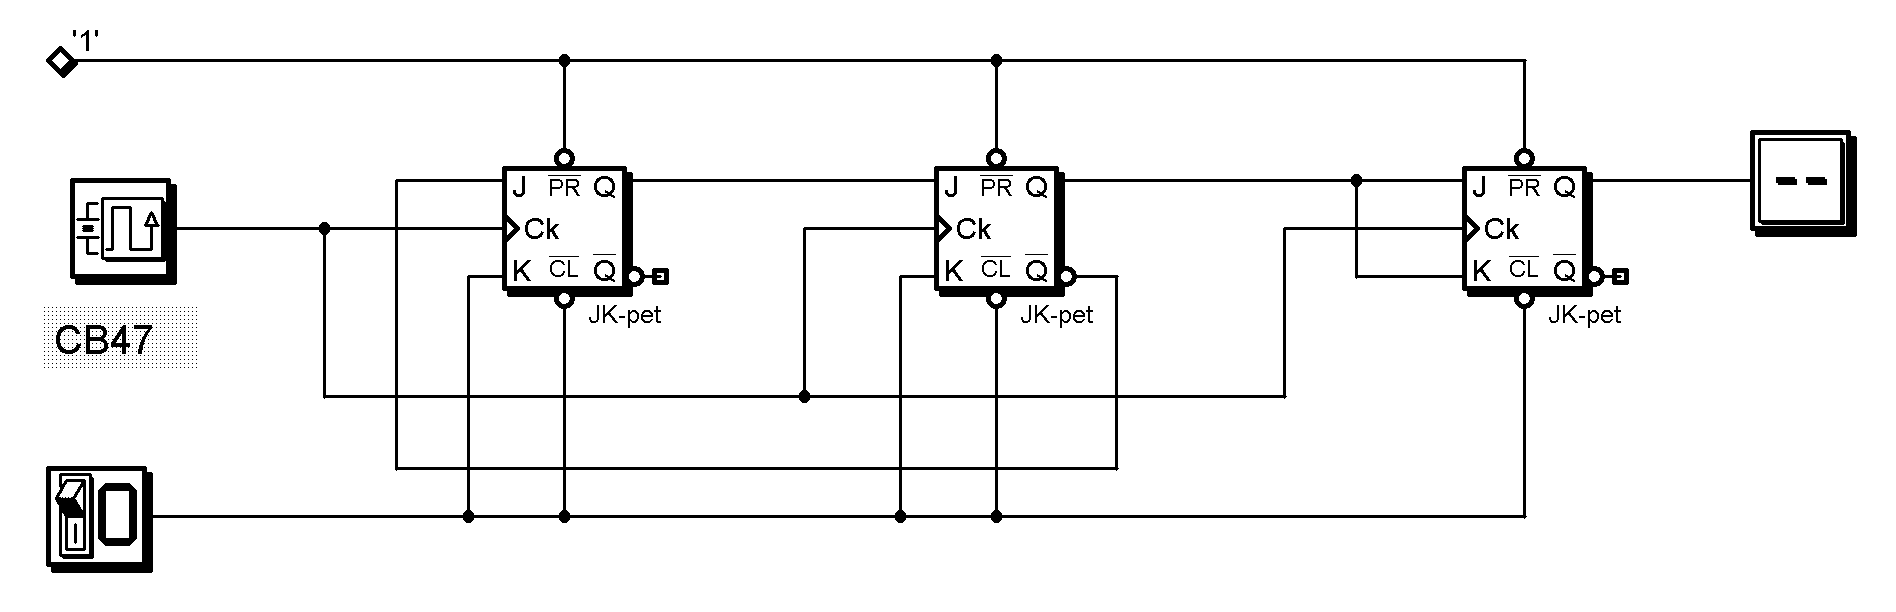
\includegraphics[width=0.9\linewidth]{./Fig_prov_div6_sincrono}
\caption{Divisore per sei sincrono.}
\label{fig:Fig_prov_div6_sincrono}
\end{figure}


\subsection{Hm.4}
Si consideri il circuito in figura \ref{fig:div5}. Calcolando la tavola di verità è possibile intuire che si tratta di un divisore per 5 con duty cycle $2/5$, come si vede in tabella \ref{tab:div5}. La tabella è stata ottenuta prendendo come stato iniziale la terna (J1, K1, Q1) = (1,1,1), dal momento che tenendo conto del numero di ingressi e uscite e delle loro relazioni il circuito presenta 3 gradi di libertà.

\begin{figure}[htp]
\centering
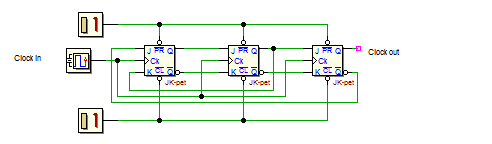
\includegraphics[scale=.8]{hm4}
\caption{Schema divisore per 5}
\label{fig:div5}
\end{figure}

\begin{table}[htp]
\centering
\caption{Tavola del divisore per 5}
\label{tab:div5}
\begin{tabular}{c|c|c|c|c|c|c|c|c|c}

\textbf{J1} & \textbf{K1} & \textbf{Q1} & \textbf{J2} & \textbf{K2} & \textbf{Q2} & \textbf{J3 }& \textbf{K3} & \textbf{Q3} & Clock \\ 
\hline
1 & 1 & 1 & 1 & 0 & 1 & 1 & 0 & 0 & $\uparrow$ \\ 
 
0 & 1 & 0 & 0 & 1 & 1 & 1 & 0 & 1 & $\downarrow$ \\ 

0 & 1 & 0 & 0 & 1 & 1 & 1 & 0 & 1 & $\uparrow$ \\ 
 
0 & 0 & 0 & 0 & 1 & 0 & 0 & 1 & 1 & $\downarrow$ \\ 

0 & 0 & 0 & 0 & 1 & 0 & 0 & 1 & 1 & $\uparrow$ \\ 
 
1 & 0 & 0 & 0 & 1 & 0 & 0 & 1 & 0 & $\downarrow$ \\ 

1 & 0 & 0 & 0 & 1 & 0 & 0 & 1 & 0 & $\uparrow$ \\ 

1 & 0 & 1 & 1 & 0 & 0 & 0 & 1 & 0 & $\downarrow$ \\ 

1 & 0 & 1 & 1 & 0 & 0 & 0 & 1 & 0 & $\uparrow$ \\ 
 
1 & 1 & 1 & 1 & 0 & 1 & 1 & 0 & 0 & $\downarrow$ \\ 

1 & 1 & 1 & 1 & 0 & 1 & 1 & 0 & 0 & $\uparrow$ \\ 

0 & 1 & 0 & 0 & 1 & 1 & 1 & 0 & 1 & $\downarrow$ \\ 
\hline 
\end{tabular} 
\end{table}
~\\

Sempre dalla tabella si vede che durante il ciclo compaiono 5 degli 8 stati (J1, K1, Q1) possibili, pertanto gli eventuali stati irraggiungibili o inutilizzati vanno da ricercarsi nei 3 assenti. Calcolando la tavola di verità si verifica che sono tutti stati inutilizzati.

\subsection{Hm. 5}

Si consideri il circuito in figura \ref{fig:count3}. Come si evince simulandolo con deeds o calcolandone la tavola di verità (tabella) esso rappresenta un contatore a 3 bit. Essendo un circuito con 3 gradi di libertà e dal momento che le uscite possibili sono 8, tanti quanti i possibili stati iniziali, non ci saranno stati irraggiungibili o inutilizzati.

\begin{figure}[htp]
\centering
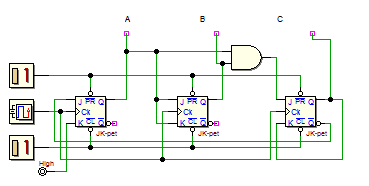
\includegraphics[scale=.8]{hm5}
\caption{Schema contatore a 3 bit}
\label{fig:count3}
\end{figure}

\begin{table}[htp]
\centering
\caption{Tavola del contatore per 3}
\label{tab:count3}
\begin{tabular}{c|c|c|c|c|c|c|c|c|c}

\textbf{J1} & \textbf{K1} &\textbf{ J2} & \textbf{K2} & \textbf{J3} & \textbf{K3} & \textbf{Q3} & \textbf{Q2} & \textbf{Q1} & Clock \\ 
\hline
1 & 1 & 1 & 1 & 0 & 0 & 0 & 0 & 1 & $\downarrow$ \\ 

1 & 1 & 1 & 1 & 0 & 0 & 0 & 0 & 1 & $\uparrow$ \\ 
 
1 & 1 & 0 & 0 & 0 & 0 & 0 & 1 & 0 & $\downarrow$ \\ 
 
1 & 1 & 0 & 0 & 0 & 0 & 0 & 1 & 0 & $\uparrow$ \\ 

1 & 1 & 1 & 1 & 1 & 0 & 0 & 1 & 1 & $\downarrow$ \\ 

1 & 1 & 1 & 1 & 1 & 0 & 0 & 1 & 1 & $\uparrow$ \\ 

0 & 1 & 0 & 0 & 0 & 1 & 1 & 0 & 0 & $\downarrow$ \\ 
 
0 & 1 & 0 & 0 & 0 & 1 & 1 & 0 & 0 & $\uparrow$ \\ 
 
1 & 1 & 0 & 0 & 0 & 0 & 0 & 0 & 0 & $\downarrow$ \\ 
 
1 & 1 & 0 & 0 & 0 & 0 & 0 & 0 & 0 & $\uparrow$ \\ 
\hline
\end{tabular} 
\end{table}
~\\

La disposizione delle uscite è scelta per rendere più evidente il comportamento del circuito come contatore per 3.

\subsection{Hm.6}

Si consideri il circuito in figura \ref{fig:contcazzodicane}. Se si legge la sequenza degli stati dalla tavola di verità in tabella \ref{tab:countcazzodicane}, si ha che il circuito fornisce come output la sequenza, in binario, (0,1,2,5,6). Quindi non tutti gli stati entrano nel ciclo del circuito. Infatti calcolando la tavola di verità per gli stati (Q3, Q2, Q1) corrispondenti a 3, 4 e 7 si ottiene che i primi due sono stati irraggiungibili, mentre il terzo è inutilizzato. Si è usato per la tavola di verità lo stesso ordine del caso precedente.

\begin{figure}[htp]
\centering
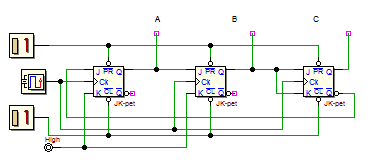
\includegraphics[scale=.8]{hm6}
\caption{Schema del ''contatore a salti''}
\label{fig:contcazzodicane}
\end{figure}

\begin{table}[htp]
\centering
\caption{Tavola del ''contatore a salti''}
\label{tab:countcazzodicane}
\begin{tabular}{c|c|c|c|c|c|c|c|c|c}

\textbf{J1} &\textbf{ K1} & \textbf{J2} & \textbf{K2} & \textbf{J3} & \textbf{K3 }& \textbf{Q3} &\textbf{ Q2} & \textbf{Q1} & Clock \\ 
\hline
1 & 1 & 1 & 1 & 0 & 0 & 0 & 0 & 1 & $\downarrow$ \\ 

1 & 1 & 1 & 1 & 0 & 0 & 0 & 0 & 1 & $\uparrow$ \\ 

1 & 1 & 0 & 1 & 1 & 1 & 0 & 1 & 0 & $\downarrow$ \\ 
 
1 & 1 & 0 & 1 & 1 & 1 & 0 & 1 & 0 & $\uparrow$ \\ 

0 & 1 & 1 & 1 & 0 & 0 & 1 & 0 & 1 & $\downarrow$ \\ 

0 & 1 & 1 & 1 & 0 & 0 & 1 & 0 & 1 & $\uparrow$ \\ 

0 & 1 & 0 & 1 & 1 & 1 & 1 & 1 & 0 & $\downarrow$ \\ 

0 & 1 & 0 & 1 & 1 & 1 & 1 & 1 & 0 & $\uparrow$ \\ 

1 & 1 & 0 & 1 & 0 & 0 & 0 & 0 & 0 & $\downarrow$ \\ 
 
1 & 1 & 0 & 1 & 0 & 0 & 0 & 0 & 0 & $\uparrow$ \\ 

1 & 1 & 1 & 1 & 0 & 0 & 0 & 0 & 1 & $\downarrow$ \\ 
\hline
\end{tabular} 
\end{table}
~\\

\subsection{Hw. 7}
Il circuito che presentiamo di seguito è certamente il più complesso fra quelli in esame: si tratta di un contatore a codifica binaria a 3 bit (capace dunque di contare da 0-8) regolabile con un apposito interruttore in modo che possa contare anche a "scendere" oltre che a "salire". Si tratta di un \textit{up-down counter}. Lo schema è riportato in Figura (\ref{fig:Fig_jk_up_down_counter_8bit}). Come si vede, la struttura che lega il secondo JK al terzo JK appare a vista modulare, cioè identicamente replicabile in serie in modo da ottenere un contatore a n-bit con facilità (per lo meno in linea teorica).\\

\begin{figure}
\centering
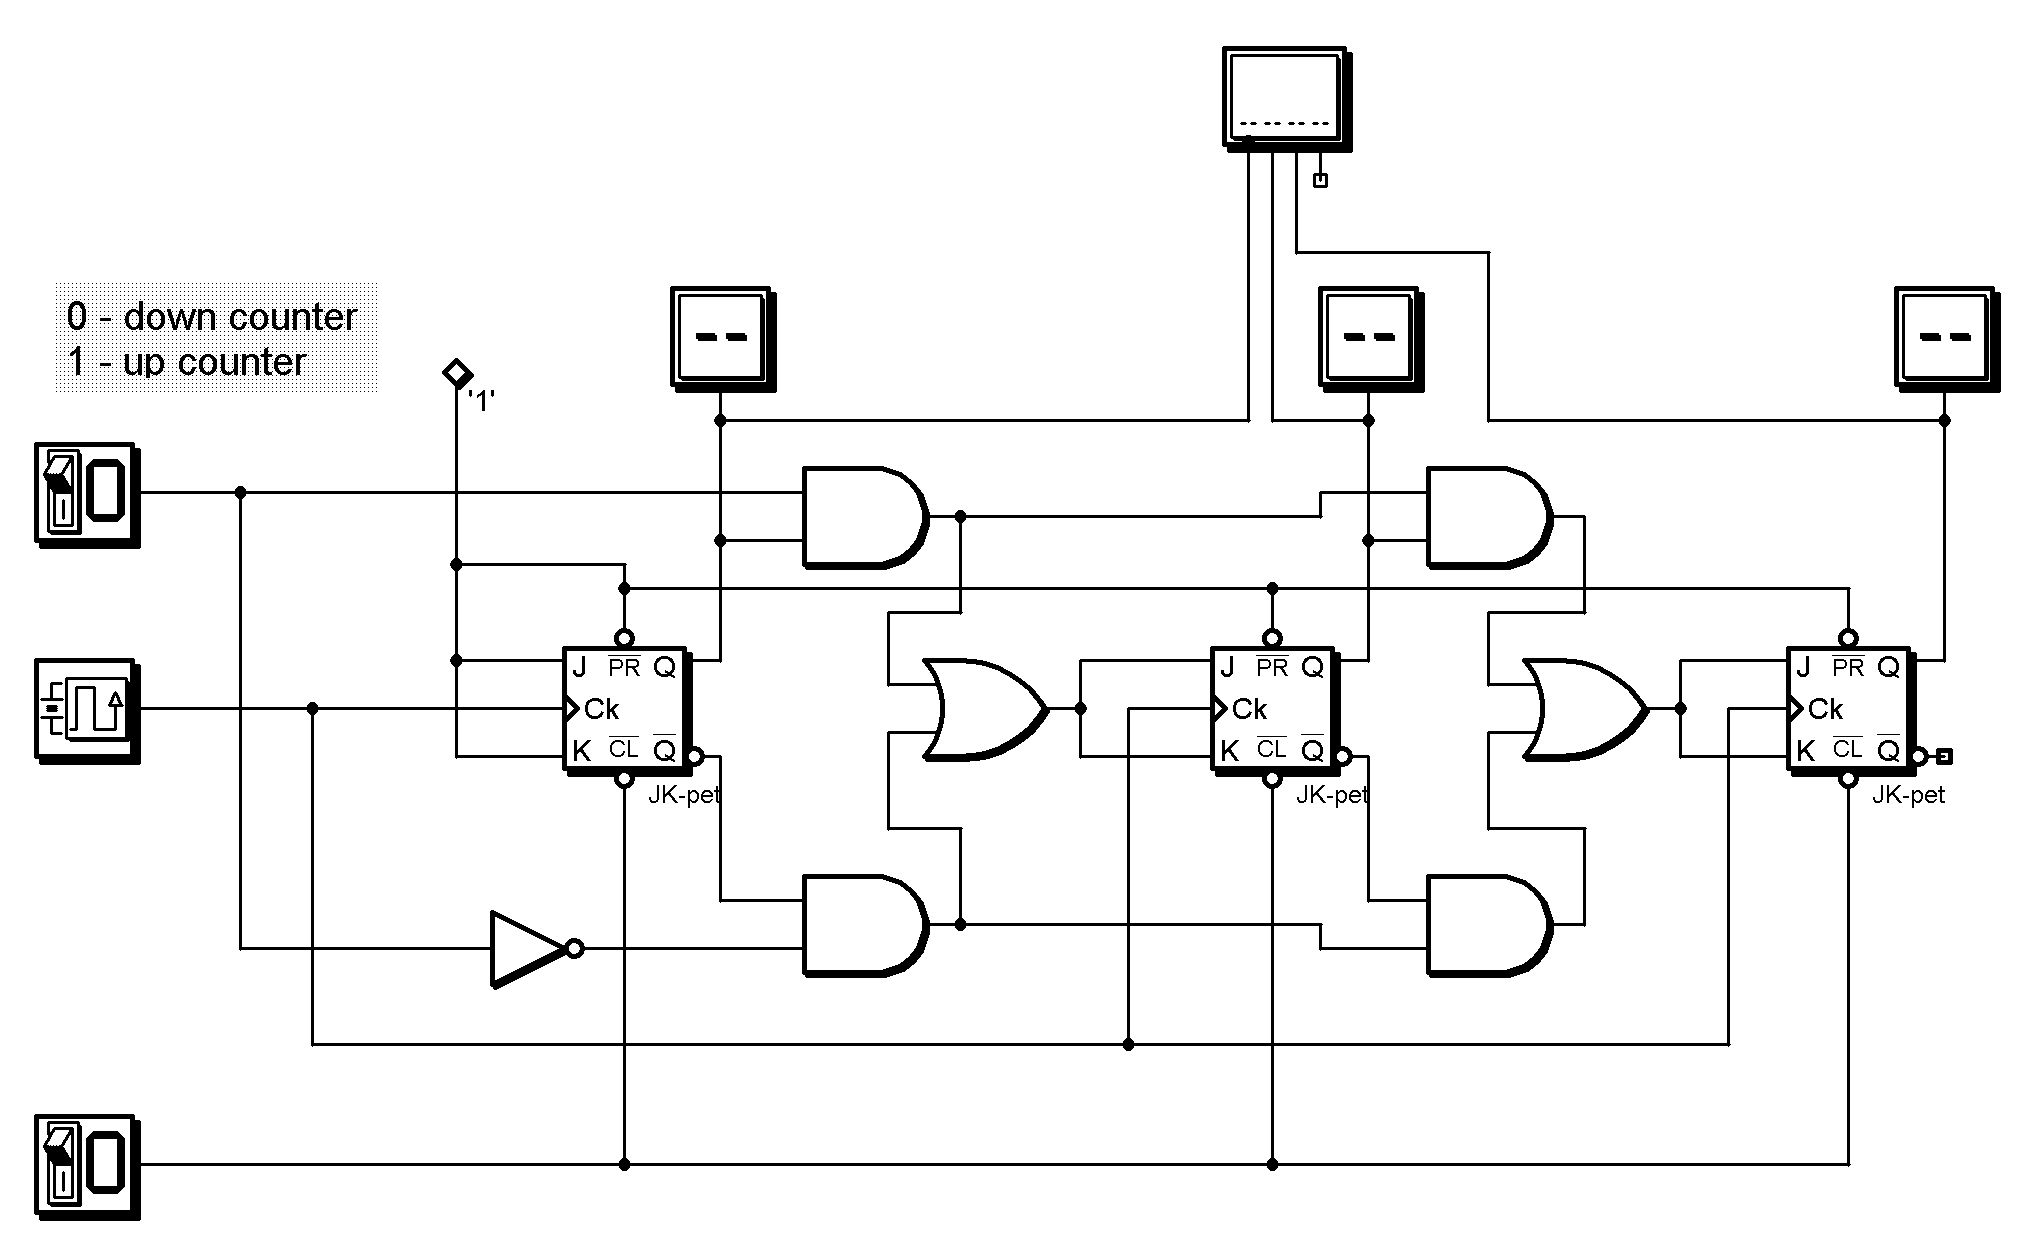
\includegraphics[width=0.8\linewidth]{./Fig_jk_up_down_counter_8bit}
\caption{Contatore decimale UP-DOWN a 8 bit}
\label{fig:Fig_jk_up_down_counter_8bit}
\end{figure}


Riportiamo di seguito la tavola di verità degli i/o dei tre integrati jk sia per la modalità di UP-counter che per quella di DOWN-counter. Come si vede tutte le triplette di stati (Q1,Q2,Q3) sono raggiunte ciclicamente. La realizzazione pratica è stata resa particolarmente difficoltosa dal non avere a disposizione dei \textbf{NOT}, \textbf{OR} e degli \textbf{AND}, per cui il numero dei circuiti \textbf{NAND} usati è cresciuto notevolmente. Nonostante questo, anche sperimentalmente siamo riusciti a ottenere un contatore UP-DOWN funzionante perfettamente e, galvanizzati dal risultato, abbiamo deciso di aggiungere un ulteriore bit (JK) al circuito per realizzare un contatore a 16 bit (0-15). Il risultato (ben funzionante, seppur poco ordinato) è riportato nell'immagine di Figura ( ) e nello schema in Figura (\ref{fig:Fig_jk_up_down_counter_16bit}).\\

%[dati_prova_hw7 ecc...]
%Figura(\ref{fig:hw7_16bit})

\begin{table}
\caption{Tavola dell'UP-counter}
\centering
\begin{tabular}{l|l|l|l|l|l|l|l|l}
\hline
\textbf{j1} & \textbf{k1} & \textbf{j2} & \textbf{k2} &\textbf{ j3} & \textbf{k3} & \textbf{q3} & \textbf{q2} & \textbf{q1} \\
\hline
1 & 1 & 1 & 1 & 0 & 0 & 0 & 0 & 1 \\
1 & 1 & 0 & 0 & 0 & 0 & 0 & 1 & 0 \\
1 & 1 & 1 & 1 & 1 & 1 & 0 & 1 & 1 \\
1 & 1 & 0 & 0 & 0 & 0 & 1 & 0 & 0 \\
1 & 1 & 1 & 1 & 0 & 0 & 1 & 0 & 1 \\
1 & 1 & 0 & 0 & 0 & 0 & 1 & 1 & 0 \\
1 & 1 & 1 & 1 & 1 & 1 & 1 & 1 & 1 \\
1 & 1 & 0 & 0 & 0 & 0 & 0 & 0 & 0 \\
\hline
\end{tabular}
\end{table}
~\\

\begin{table}
\centering
\caption{Tavola del DOWN-counter}

\begin{tabular}{l|l|l|l|l|l|l|l|l}
\hline
\textbf{j1} & \textbf{k1} & \textbf{j2} & \textbf{k2} &\textbf{ j3} & \textbf{k3} & \textbf{q3} & \textbf{q2} & \textbf{q1} \\
\hline
1 & 1 & 0 & 0 & 0 & 0 & 1 & 1 & 1 \\
1 & 1 & 1 & 1 & 0 & 0 & 1 & 1 & 0 \\
1 & 1 & 0 & 0 & 0 & 0 & 1 & 0 & 1 \\
1 & 1 & 1 & 1 & 1 & 1 & 1 & 0 & 0 \\
1 & 1 & 0 & 0 & 0 & 0 & 0 & 1 & 1 \\
1 & 1 & 1 & 1 & 0 & 0 & 0 & 1 & 0 \\
1 & 1 & 0 & 0 & 0 & 0 & 0 & 0 & 1 \\
1 & 1 & 1 & 1 & 1 & 1 & 0 & 0 & 0 \\
1 & 1 & 0 & 0 & 0 & 0 & 1 & 1 & 1 \\
\hline
\end{tabular}

\end{table}
~\\


\begin{figure}
\centering
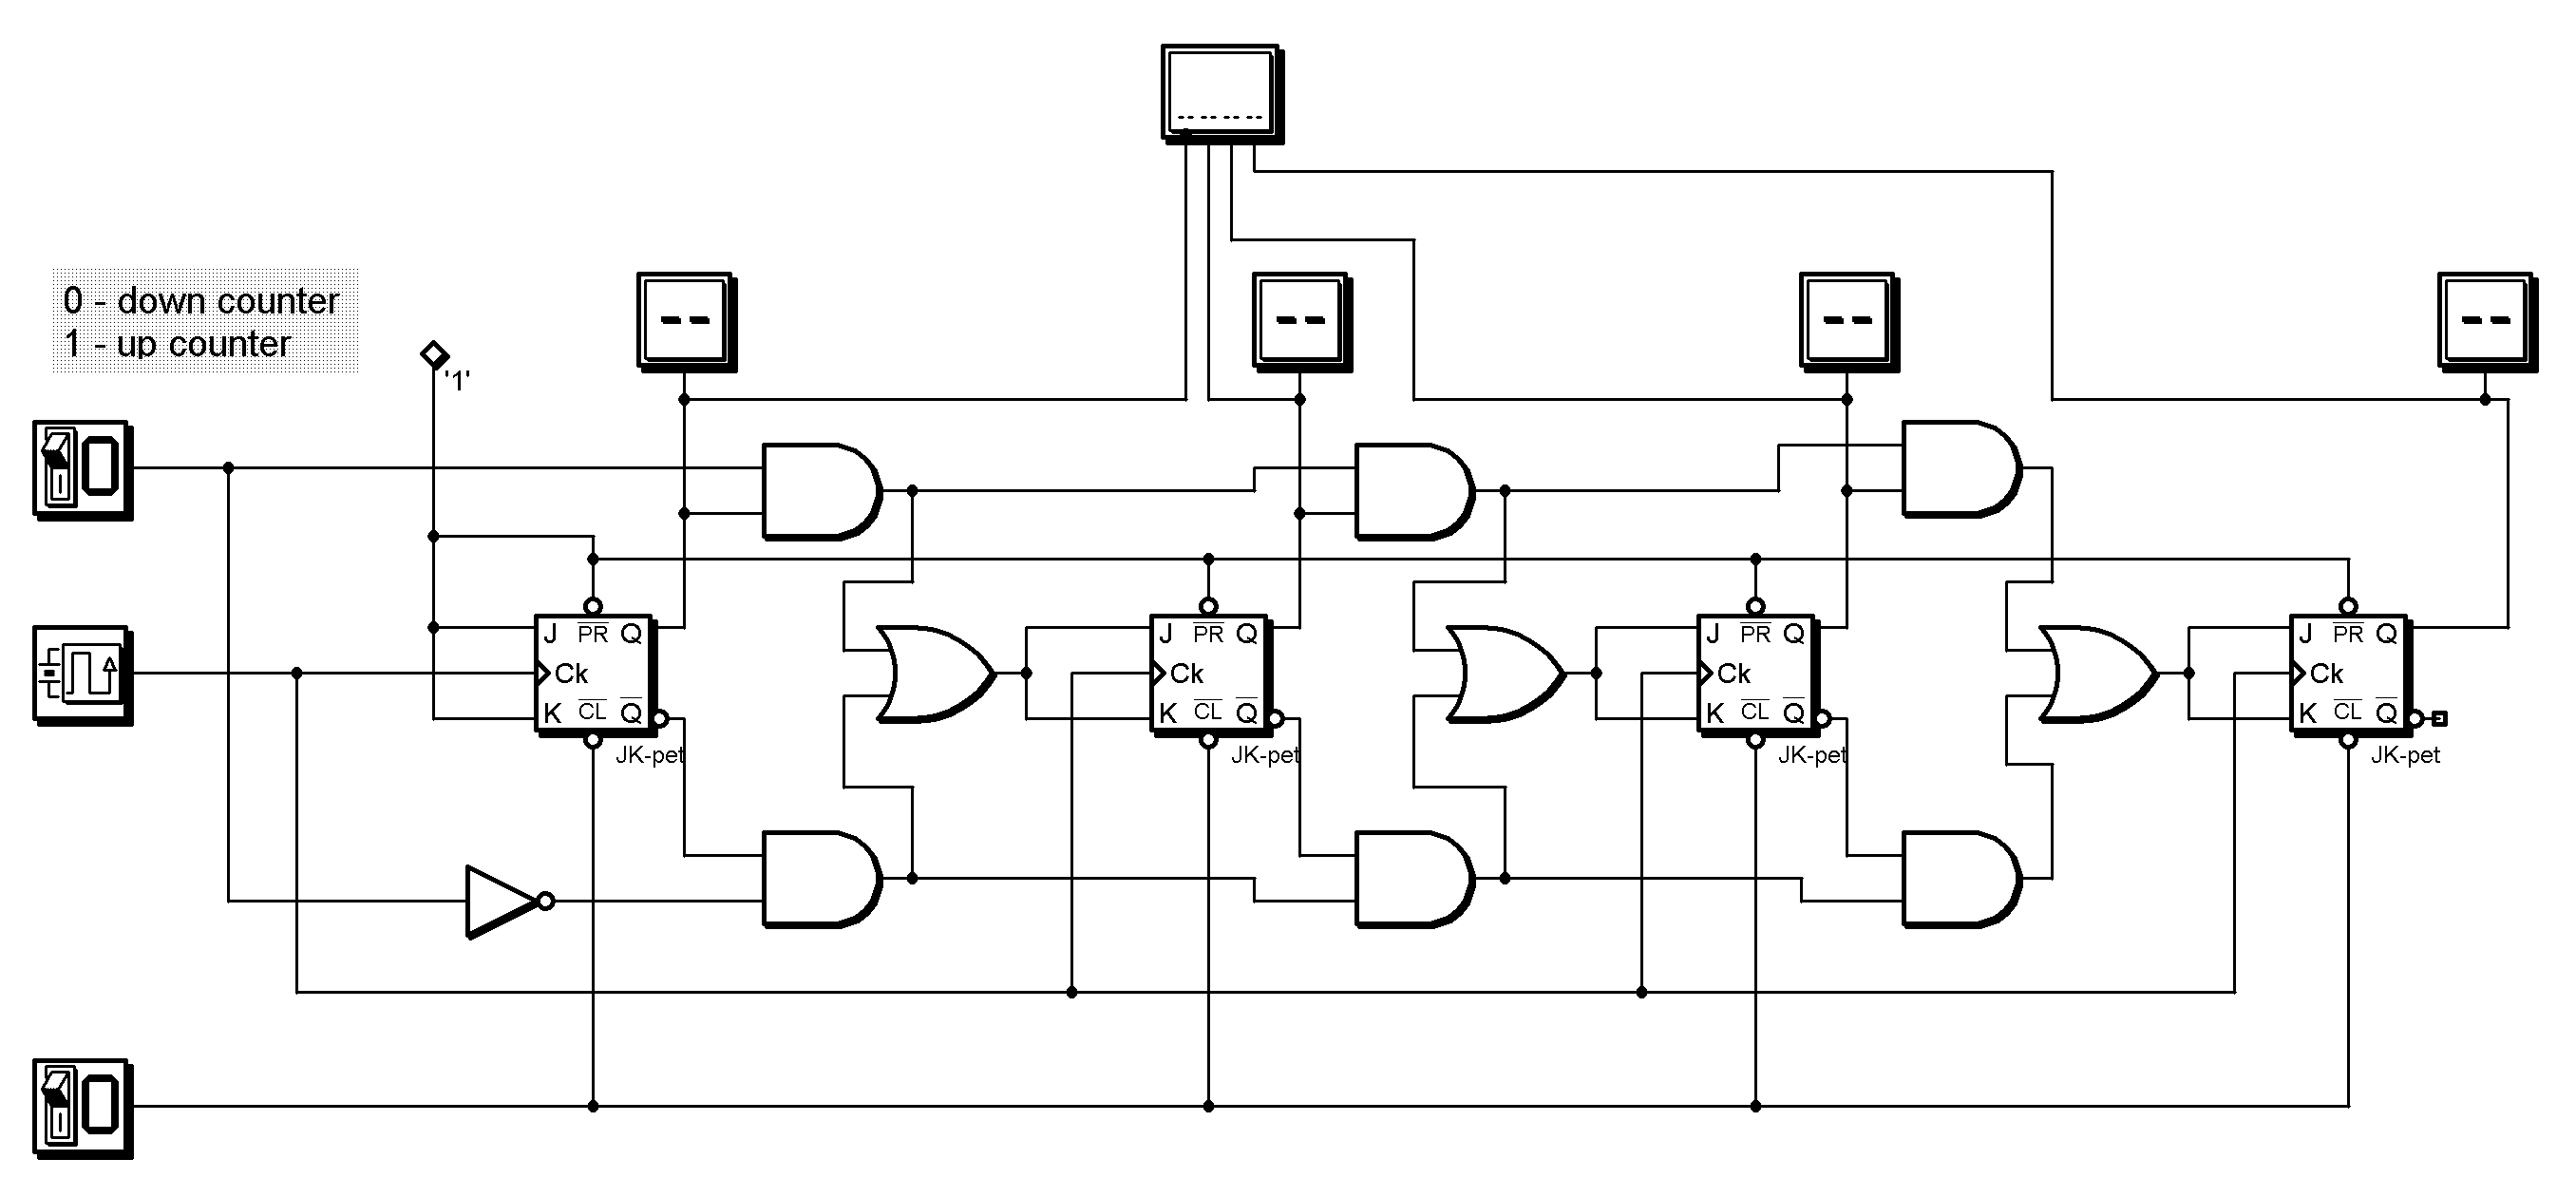
\includegraphics[width=0.9\linewidth]{./Fig_jk_up_down_counter_16bit}
\caption{Contatore decimale UP-DOWN a 16 bit}
\label{fig:Fig_jk_up_down_counter_16bit}
\end{figure}

%\begin{figure}
%\centering
%\includegraphics[width=0.9\linewidth]{./hw7_16bit}
%\caption{Contatore binario UP-DOWN a 16bit}
%\label{fig:hw7_16bit}
%\end{figure}

In entrambi i casi (8bit e 16bit), tutti gli stati sono raggiungibili (e raggiunti) circolarmente ad ogni ciclo.

\subsection{Hm. 8}

SI consideri il circuito in figura \ref{fig:count4}. Esso possiede 4 gradi di libertàe quindi ammette 16 possibili stati iniziali del tipo (Q1,Q2,Q3,Q4). In tabella \ref{tab:count4} è mostrata la tavola di verità, in cui compaino solo i J e gli stati uscenti dal clock $\uparrow$. Come si vede il circuito si comporta come un contatore a 4 bit ed esplora tutti e 16 i possibili stati. Pertanto non si hanno stati irraggiungibili o inutilizzati.

\begin{figure}[htp]
\centering
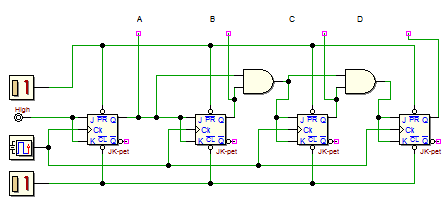
\includegraphics[scale=.8]{hm8}
\caption{Schema contatore a 4 bit}
\label{fig:count4}
\end{figure}

\begin{table}
\centering
\caption{Tavola del contatore 4 bit}
\label{tab:count4}
\begin{tabular}{c|c|c|c|c|c|c|c}
\hline 
\textbf{J1} & \textbf{J2} & \textbf{J3} & \textbf{J4} & \textbf{Q4} & \textbf{Q3} & \textbf{Q2} & \textbf{Q1} \\ 
\hline 
1 & 1 & 0 & 0 & 0 & 0 & 0 & 1 \\ 

1 & 0 & 0 & 0 & 0 & 0 & 1 & 0 \\ 
 
1 & 1 & 1 & 0 & 0 & 0 & 1 & 1 \\ 
 
1 & 0 & 0 & 0 & 0 & 1 & 0 & 0 \\ 
 
1 & 1 & 0 & 0 & 0 & 1 & 0 & 1 \\ 
 
1 & 0 & 1 & 0 & 0 & 1 & 1 & 0 \\ 

1 & 1 & 0 & 1 & 0 & 1 & 1 & 1 \\ 

1 & 0 & 0 & 0 & 1 & 0 & 0 & 0 \\ 

1 & 1 & 1 & 0 & 1 & 0 & 0 & 1 \\ 

1 & 0 & 0 & 0 & 1 & 0 & 1 & 0 \\ 

1 & 1 & 0 & 0 & 1 & 0 & 1 & 1 \\ 
 
1 & 0 & 1 & 0 & 1 & 1 & 0 & 0 \\ 

1 & 1 & 0 & 0 & 1 & 1 & 0 & 1 \\ 
 
1 & 0 & 0 & 0 & 1 & 1 & 1 & 0 \\ 
 
1 & 1 & 1 & 1 & 1 & 1 & 1 & 0 \\ 

1 & 0 & 0 & 0 & 0 & 0 & 0 & 0 \\ 
\hline 
\end{tabular}
\end{table}


\begin{thebibliography}{5}

	%Each item starts with a \bibitem{reference} command and the details thereafter.
	
	\bibitem{JH6} % Conference paper
	Product data sheet: Dual Type D Flip-Flop \textsc{mc14013b}.
	\url{http://onsemi.com}

	\bibitem{M06} % Conference paper
	Paul Horowitz, Winfield Hill - The Art of Electronics. Cambridge University Press (1989).
	
\end{thebibliography}


\end{document}